\documentclass[letterpaper,10pt,titlepage,draftclsnofoot,onecolumn,onesided] {IEEEtran}
\usepackage{listings}
\usepackage{underscore}
\usepackage[bookmarks=true]{hyperref}
\usepackage[utf8]{inputenc}
\usepackage[english]{babel}
%\usepackage{titling}
\usepackage{graphicx}
\usepackage{xcolor}
\usepackage[noadjust]{cite}
\usepackage{setspace}
\usepackage{float}
\usepackage{pdfpages}
\nocite{*}
\graphicspath{ {img/} }
%\usepackage{abstract}

\newcommand{\namesigdate}[2][4cm]{%
  \begin{tabular}{@{}p{#1}@{}}
    #2 \\[2\normalbaselineskip] \hrule \\[0pt]
    {\small \textit{Signature}} \\[2\normalbaselineskip] \hrule \\[0pt]
    {\small \textit{Date}}
  \end{tabular}
}
\newcommand{\studentnamesigdate}[2][4cm]{%
  \begin{tabular}{@{}p{#1}@{}}
    #2 \\[2\normalbaselineskip] \hrule \\[0pt]
    {\small \textit{Signature}} \\[2\normalbaselineskip] \hrule \\[0pt]
    {\small \textit{Signature}} \\[2\normalbaselineskip] \hrule \\[0pt]
    {\small \textit{Signature}} \\[2\normalbaselineskip] \hrule \\[0pt]
    {\small \textit{Signature}} \\[2\normalbaselineskip] \hrule \\[0pt]
    {\small \textit{Date}}
  \end{tabular}
}

\hypersetup{
    bookmarks=false,    % show bookmarks bar?
    pdftitle={Progress Report},    % title
    pdfauthor={Cramer Smith, Sam Lichlyter, Eric Winkler, Zach Schneider},                     % author
    pdfsubject={Progress Report},                        % subject of the document
    pdfkeywords={IFT, Report, Postal}, % list of keywords
    colorlinks=true,       % false: boxed links; true: colored links
    linkcolor=black,       % color of internal links
    citecolor=black,       % color of links to bibliography
    filecolor=black,        % color of file links
    urlcolor=blue,        % color of external links
    linktoc=page            % only page is linked
} 

\lstdefinestyle{customperl}{
  belowcaptionskip=1\baselineskip,
  breaklines=true,
  frame=L,
  xleftmargin=\parindent,
  language=Perl,
  columns=fullflexible,
  showstringspaces=false,
  basicstyle=\footnotesize\ttfamily,
  keywordstyle=\bfseries\color{green!40!black},
  commentstyle=\itshape\color{purple!40!black},
  identifierstyle=\color{blue},
  stringstyle=\color{orange},
  numbers=left
}
\lstset{escapechar=@, style=customperl}

\begin{document}

% Cover Page

\includepdf[pages={-}]{coverpage.pdf}
\tableofcontents


\pagebreak

\section{Introduction}
\subsection{Client and Project Origins}
This project originated in August 2016 when one of the the team's members, Sam Lichlyter, was made aware of a research opportunity offered by Professor Christopher Scaffidi from Oregon State University. 
Prof. Scaffidi's primary research area is in Information Foraging Theory (IFT) which revolves around studying how humans find and utilize information sources. 
Sam, already a student researcher under Prof. Scaffidi, asked if he could create a Senior Capstone project out of IFT in a new study concerning software developers.
Prof. Scaffidi prompted Sam to identify a team and to come up with a project proposal that would develop a software tool according to the principles of IFT. 
Sam included Eric Winkler, Zach Schneider and Cramer Smith in the potential Capstone team. 
There were two proposals submitted for consideration: an interface to allow developers to read and search program log files more easily, and an extension for an integrated development environment (IDE) that would automatically organize a developer's code into appropriate concerns i.e., the data layer, interface layer, and application layer.
The latter of the proposals was selected and this Capstone team was formed to undertake it.

\subsection{Project Purpose and Expectations}
A more detailed explanation of what the team was tasked with doing is as follows.
First, design a tool according to IFT design patterns that will help developers find and utilize information, in this case, within an IDE.
Second, build and code said tool until it is in a state where it is useful in its main purposes.
Next, organize a series of formal user tests to determine if the tool aides developers in performing a set of real world tasks.
Finally, analyze the results of the tests and, if the results are positive, write a formal research paper describing the entire process and its relationship to IFT.
Prof. Scaffidi supervised the design process in the Fall. The team met with him about once and month to check in and discuss any design questions or changes. 
Emails were exchanged a bit more often. 
He left the coding and implementation phase largely up to the team during the end of the Fall through the Winter and contact was infrequent. 
Spring term saw contact pick up again as the team finalized the product with him and began arranging the necessary materials for user testing. 
Prof. Scaffidi has and will continue to directly facilitate the actual testing and analysis process until it is complete.

\subsection{Project Roles}
Throughout the year, each team member assumed and carried out various roles depending on the stage of the project. 
Every member generally contributed to all aspects of the project, but the responsibility for some areas was assumed primarily by one individual.

Sam served as the team's primary client contact since the relationship had existed prior to the beginning of this project. 
He had a major role in the design and implementation of the parser component of this tool, along with Eric. 
Additionally, Sam wrote many of the grammars and rules that the parser would use to find specific data within developers' codebases. 

Zach took primary responsibility for project documentation, deadlines and general administrative work. He contributed to early iterations of the data structure used to store parsed data within the tool. 
He then transitioned to adding features to the user interface (UI) and testing various use cases within it.

Cramer did much of the research into which IDE the tool would be developed for. 
Once Visual Studio Code was decided upon by the team as the platform for this project, he also created the core of code required to launch and include extensions within that platform. 
Cramer deployed each iteration of the tool to the Microsoft VS Code Extension Gallery online when various project milestones were reached.

Eric served as overall project architect, coming up with the general structure of the project from the original proposal and changing it as necessary throughout the year. 
He worked with Sam in building the parser and created the core of the UI and Electron window code. 
When the parser was modified in the middle of the year, he also re-worked the data structure system being used. \\


\section{Original Requirements and Timeline}
The original Requirements Document for this project is inserted in the following pages.

\includepdf[pages={-}]{requirements.pdf}
\pagebreak
\section{Updates to Requirements and Timeline}
Below is a simplified list of all requirements for this project as of the final Requirements document submitted on November 4th, 2016. 
No changes to requirements were made for the duration of the project.
\subsection{Product Functions}
\small{
\begin{center}
	\begin{singlespace}
		\begin{tabular}{ |  p{0.25\linewidth}  |  p{0.25\linewidth}  | p{0.25\linewidth} | p{0.25\linewidth} |}
		\hline
		0 & Requirement & Changes & Comments \\ \hline
		
			1
		& 
			\begin{itemize}
				\item Offered in a free, cross-platform text editor
			\end{itemize}
		& 
			\begin{itemize}
				\item None
			\end{itemize}
		&
			\begin{itemize}
				\item Completed
			\end{itemize} 
		
        \\ \hline

			2
		& 
			\begin{itemize}
				\item Provide the user with a visual perspective of their project
			\end{itemize}
		& 
			\begin{itemize}
				\item None
			\end{itemize}
		&
			\begin{itemize}
				\item Completed
			\end{itemize} 
		
        \\ \hline

            3
		& 
			\begin{itemize}
				\item Parse project for bad coding practice/incorrect formatting
			\end{itemize}
		& 
			\begin{itemize}
				\item None
			\end{itemize}
		&
			\begin{itemize}
				\item Completed. This is implemented through the Notifications/Error grammars.
			\end{itemize} 
		
        \\ \hline

            4
		& 
			\begin{itemize}
				\item Indicate to user when \"errors\" are parsed
			\end{itemize}
		& 
			\begin{itemize}
				\item None
			\end{itemize}
		&
			\begin{itemize}
				\item Completed. Mid-winter we began to refer to errors by a more appropriate name: Notifications. 
                The functionality remained unchanged.
			\end{itemize} 
		
        \\ \hline

        	5
		& 
			\begin{itemize}
				\item Visually display links between files
			\end{itemize}
		& 
			\begin{itemize}
				\item None
			\end{itemize}
		&
			\begin{itemize}
				\item Completed
			\end{itemize} 
		
        \\ \hline

        	6
		& 
			\begin{itemize}
				\item Rules defined by user defined grammars
			\end{itemize}
		& 
			\begin{itemize}
				\item In an earlier, pre-final version of the requirements documents, rules were defined by W3 best practices for web projects.
                This changed by the time of the final submission on November 4th to rules being defined by user grammars.
			\end{itemize}
		&
			\begin{itemize}
				\item Completed
			\end{itemize} 
		
        \\ \hline

        	7
		& 
			\begin{itemize}
				\item Ignore lines of code marked in an exception list
			\end{itemize}
		& 
			\begin{itemize}
				\item None
			\end{itemize}
		&
			\begin{itemize}
				\item Completed. Implemented through comment grammars and the postal.ignore functionality.
			\end{itemize} 
		
        \\ \hline

        	8
		& 
			\begin{itemize}
				\item Parse projects up to 100,000 LOC with less than one second of lag
			\end{itemize}
		& 
			\begin{itemize}
				\item None
			\end{itemize}
		&
			\begin{itemize}
				\item This requirement is situationally completed. 
                It does work for projects of 100,000 lines but will have problems with individual files of that size.
			\end{itemize} 
		
        \\ \hline
		\end{tabular}
	\end{singlespace}
\end{center}
}
\subsection{External Interfaces}
\small{
\begin{center}
	\begin{singlespace}
		\begin{tabular}{ |  p{0.25\linewidth}  |  p{0.25\linewidth}  | p{0.25\linewidth} | p{0.25\linewidth} |}
		\hline
		0 & Requirement & Changes & Comments \\ \hline
		
			1
		& 
			\begin{itemize}
				\item Two main elements: File Map UI and Error List
			\end{itemize}
		& 
			\begin{itemize}
				\item None, some additionally functionality was added.
			\end{itemize}
		&
			\begin{itemize}
				\item Completed. Error List now refereed to as Notification List
			\end{itemize} 
		
        \\ \hline

			2
		& 
			\begin{itemize}
				\item Toolbar for options
			\end{itemize}
		& 
			\begin{itemize}
				\item None
			\end{itemize}
		&
			\begin{itemize}
				\item Completed
			\end{itemize} 
		
        \\ \hline

            3
		& 
			\begin{itemize}
				\item Populate File Map with contents of opened solution
			\end{itemize}
		& 
			\begin{itemize}
				\item None
			\end{itemize}
		&
			\begin{itemize}
				\item Completed. This is implemented through the Notifications/Error grammars.
			\end{itemize} 
		
        \\ \hline

            4
		& 
			\begin{itemize}
				\item Visual indicator of links and errors
			\end{itemize}
		& 
			\begin{itemize}
				\item None
			\end{itemize}
		&
			\begin{itemize}
				\item Completed
			\end{itemize} 
		
        \\ \hline

        	5
		& 
			\begin{itemize}
				\item "Dig down" into a file to identify sub-nodes
			\end{itemize}
		& 
			\begin{itemize}
				\item None
			\end{itemize}
		&
			\begin{itemize}
				\item Completed
			\end{itemize} 
		
        \\ \hline

        	6
		& 
			\begin{itemize}
				\item Error list displays all errors parsed
			\end{itemize}
		& 
			\begin{itemize}
				\item None
			\end{itemize}
		&
			\begin{itemize}
				\item Completed
			\end{itemize} 
		
        \\ \hline

        	7
		& 
			\begin{itemize}
				\item User can click error to navigate to corresponding location in code
			\end{itemize}
		& 
			\begin{itemize}
				\item None
			\end{itemize}
		&
			\begin{itemize}
				\item Completed, Implemented through double clicking a node
			\end{itemize} 
		
        \\ \hline

        	8
		& 
			\begin{itemize}
				\item User can hover over error and will highlight location in File Map
			\end{itemize}
		& 
			\begin{itemize}
				\item None
			\end{itemize}
		&
			\begin{itemize}
				\item Completed
			\end{itemize} 
		
        \\ \hline
		\end{tabular}
	\end{singlespace}
\end{center}
}

\subsection{Functions}
\small{
\begin{center}
	\begin{singlespace}
		\begin{tabular}{ |  p{0.25\linewidth}  |  p{0.25\linewidth}  | p{0.25\linewidth} | p{0.25\linewidth} |}
		\hline
		0 & Requirement & Changes & Comments \\ \hline
		
			1
		& 
			\begin{itemize}
				\item Be able to parse JavaScript, HTML and CSS
			\end{itemize}
		& 
			\begin{itemize}
				\item None
			\end{itemize}
		&
			\begin{itemize}
				\item Completed, implemented through user grammars
			\end{itemize} 
		
        \\ \hline

		\end{tabular}
	\end{singlespace}
\end{center}
}

\subsection{Performance Requirements}
\small{
\begin{center}
	\begin{singlespace}
		\begin{tabular}{ |  p{0.25\linewidth}  |  p{0.25\linewidth}  | p{0.25\linewidth} | p{0.25\linewidth} |}
		\hline
		0 & Requirement & Changes & Comments \\ \hline
		
			1
		& 
			\begin{itemize}
				\item 30 HTML, 5 CSS, 10 JS files in less than one second
			\end{itemize}
		& 
			\begin{itemize}
				\item None
			\end{itemize}
		&
			\begin{itemize}
				\item Completed
			\end{itemize} 
		
        \\ \hline

		\end{tabular}
	\end{singlespace}
\end{center}
}


\subsection{Software System Attributes}
\small{
\begin{center}
	\begin{singlespace}
		\begin{tabular}{ |  p{0.25\linewidth}  |  p{0.25\linewidth}  | p{0.25\linewidth} | p{0.25\linewidth} |}
		\hline
		0 & Requirement & Changes & Comments \\ \hline
		
			1
		& 
			\begin{itemize}
				\item Available on VS Code Extension Marketplace
			\end{itemize}
		& 
			\begin{itemize}
				\item None
			\end{itemize}
		&
			\begin{itemize}
				\item Completed
			\end{itemize} 
		
        \\ \hline

		\end{tabular}
	\end{singlespace}
\end{center}
}

\subsection{Gantt of Implementation Progress for the Year}
\begin{figure}[H]
	\centering
	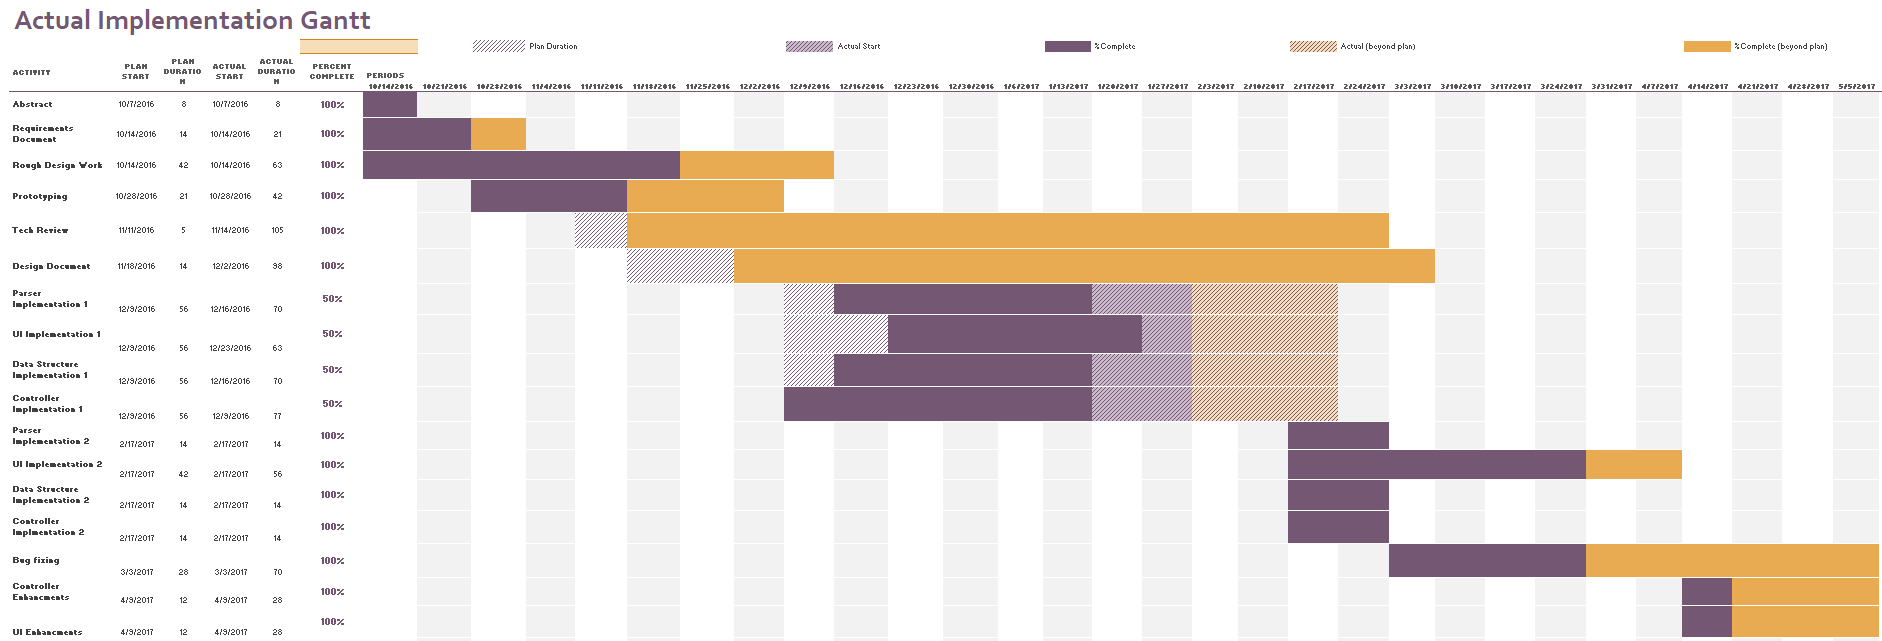
\includegraphics[width=1.1\textwidth]{Gantt}
	\caption{Gantt of the implementation progress for the academic year.}
\end{figure}
\begin{figure}[H]
	\centering
	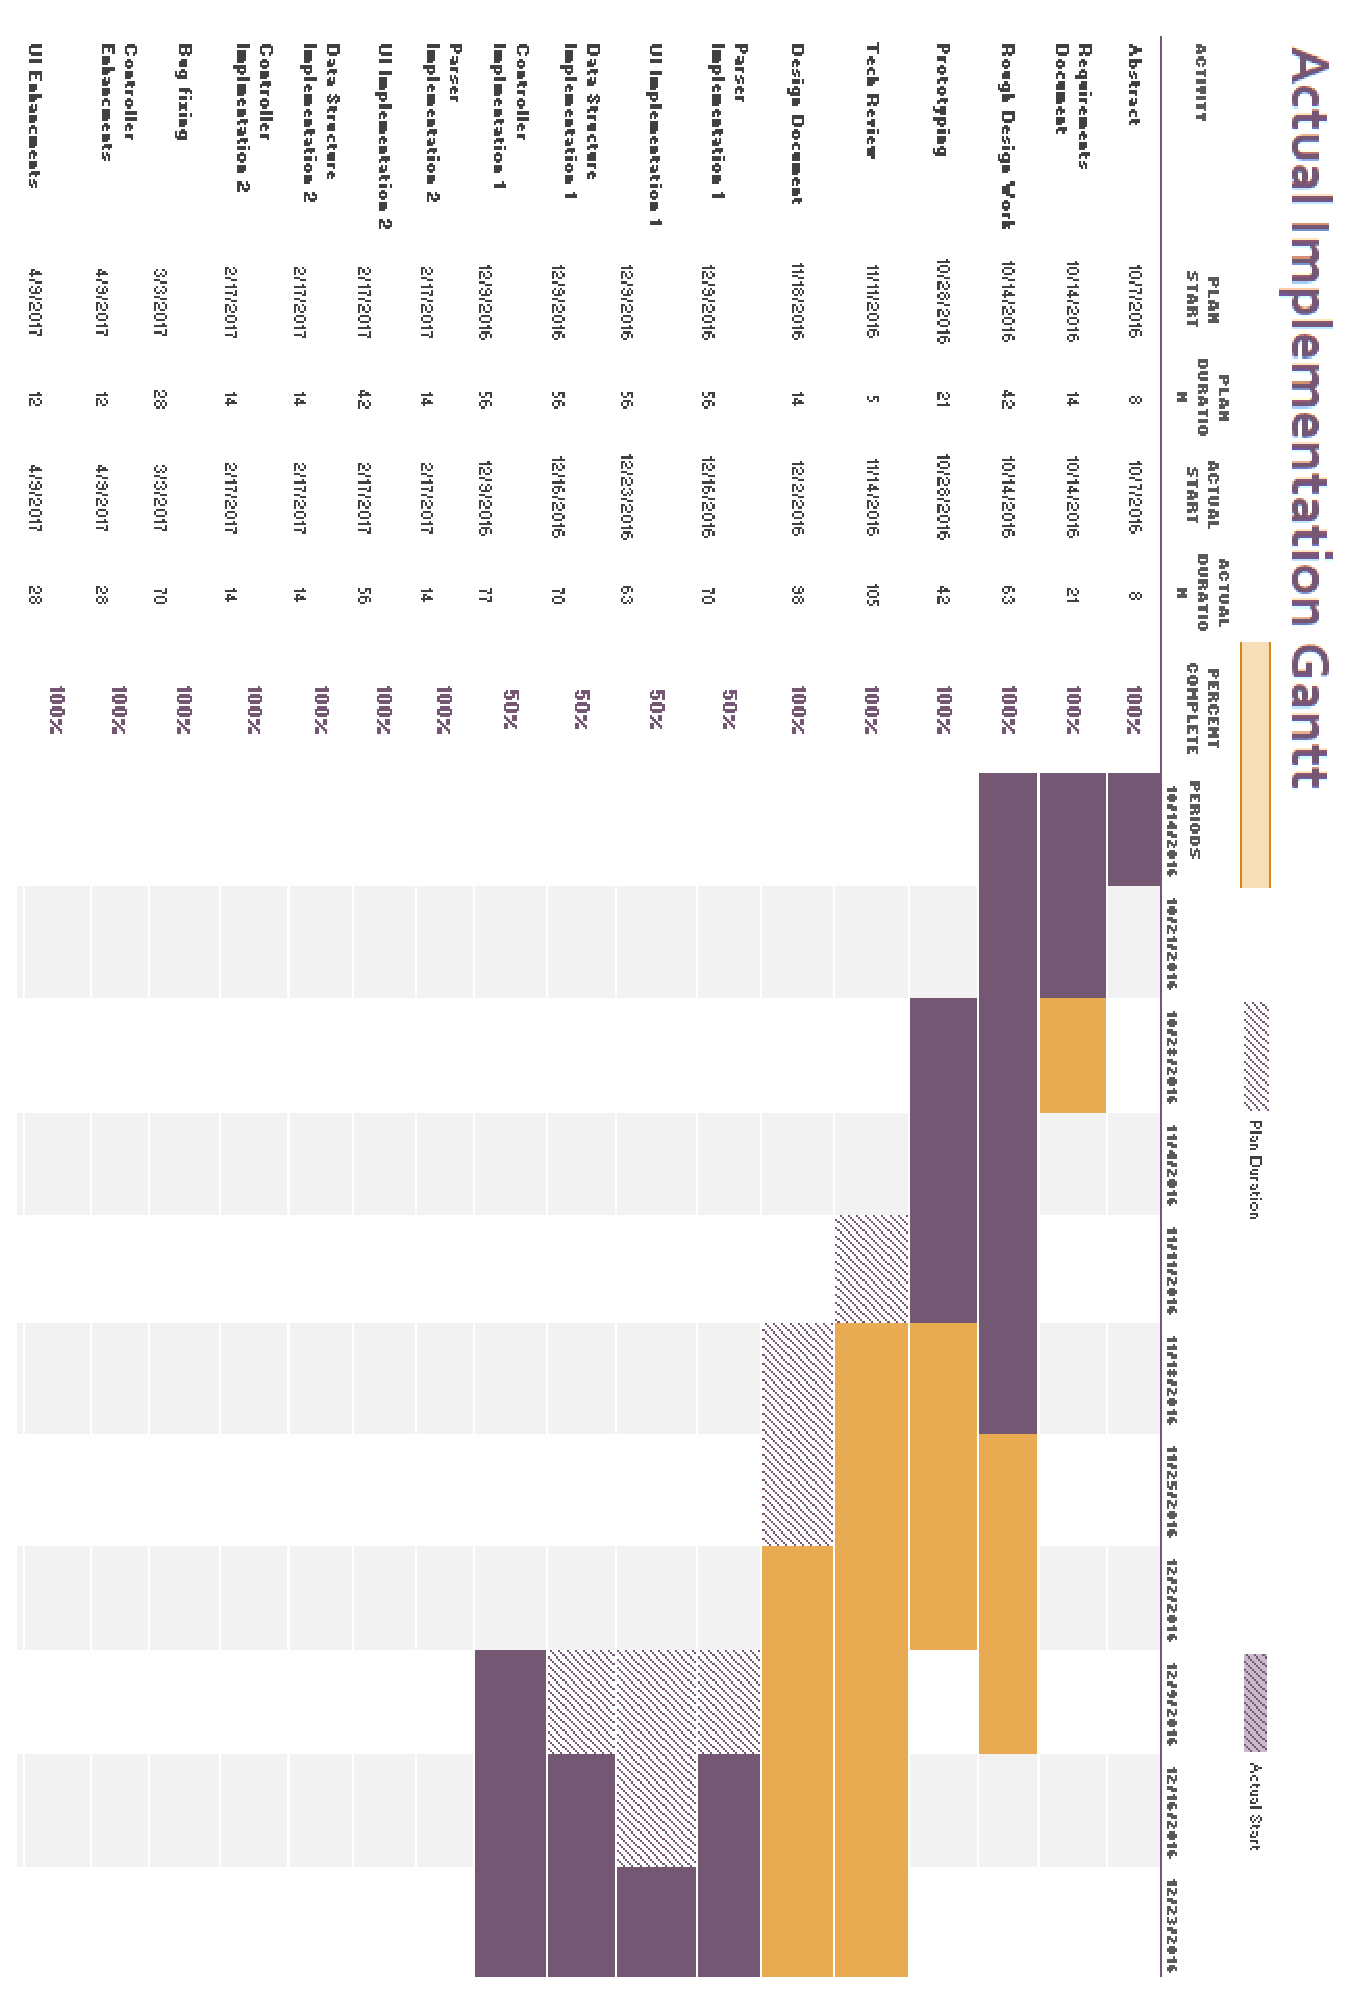
\includegraphics[width=.95\textwidth]{GanttTop}
	\caption{Top half of the Gantt for readability.}
\end{figure}
\begin{figure}[H]
	\centering
	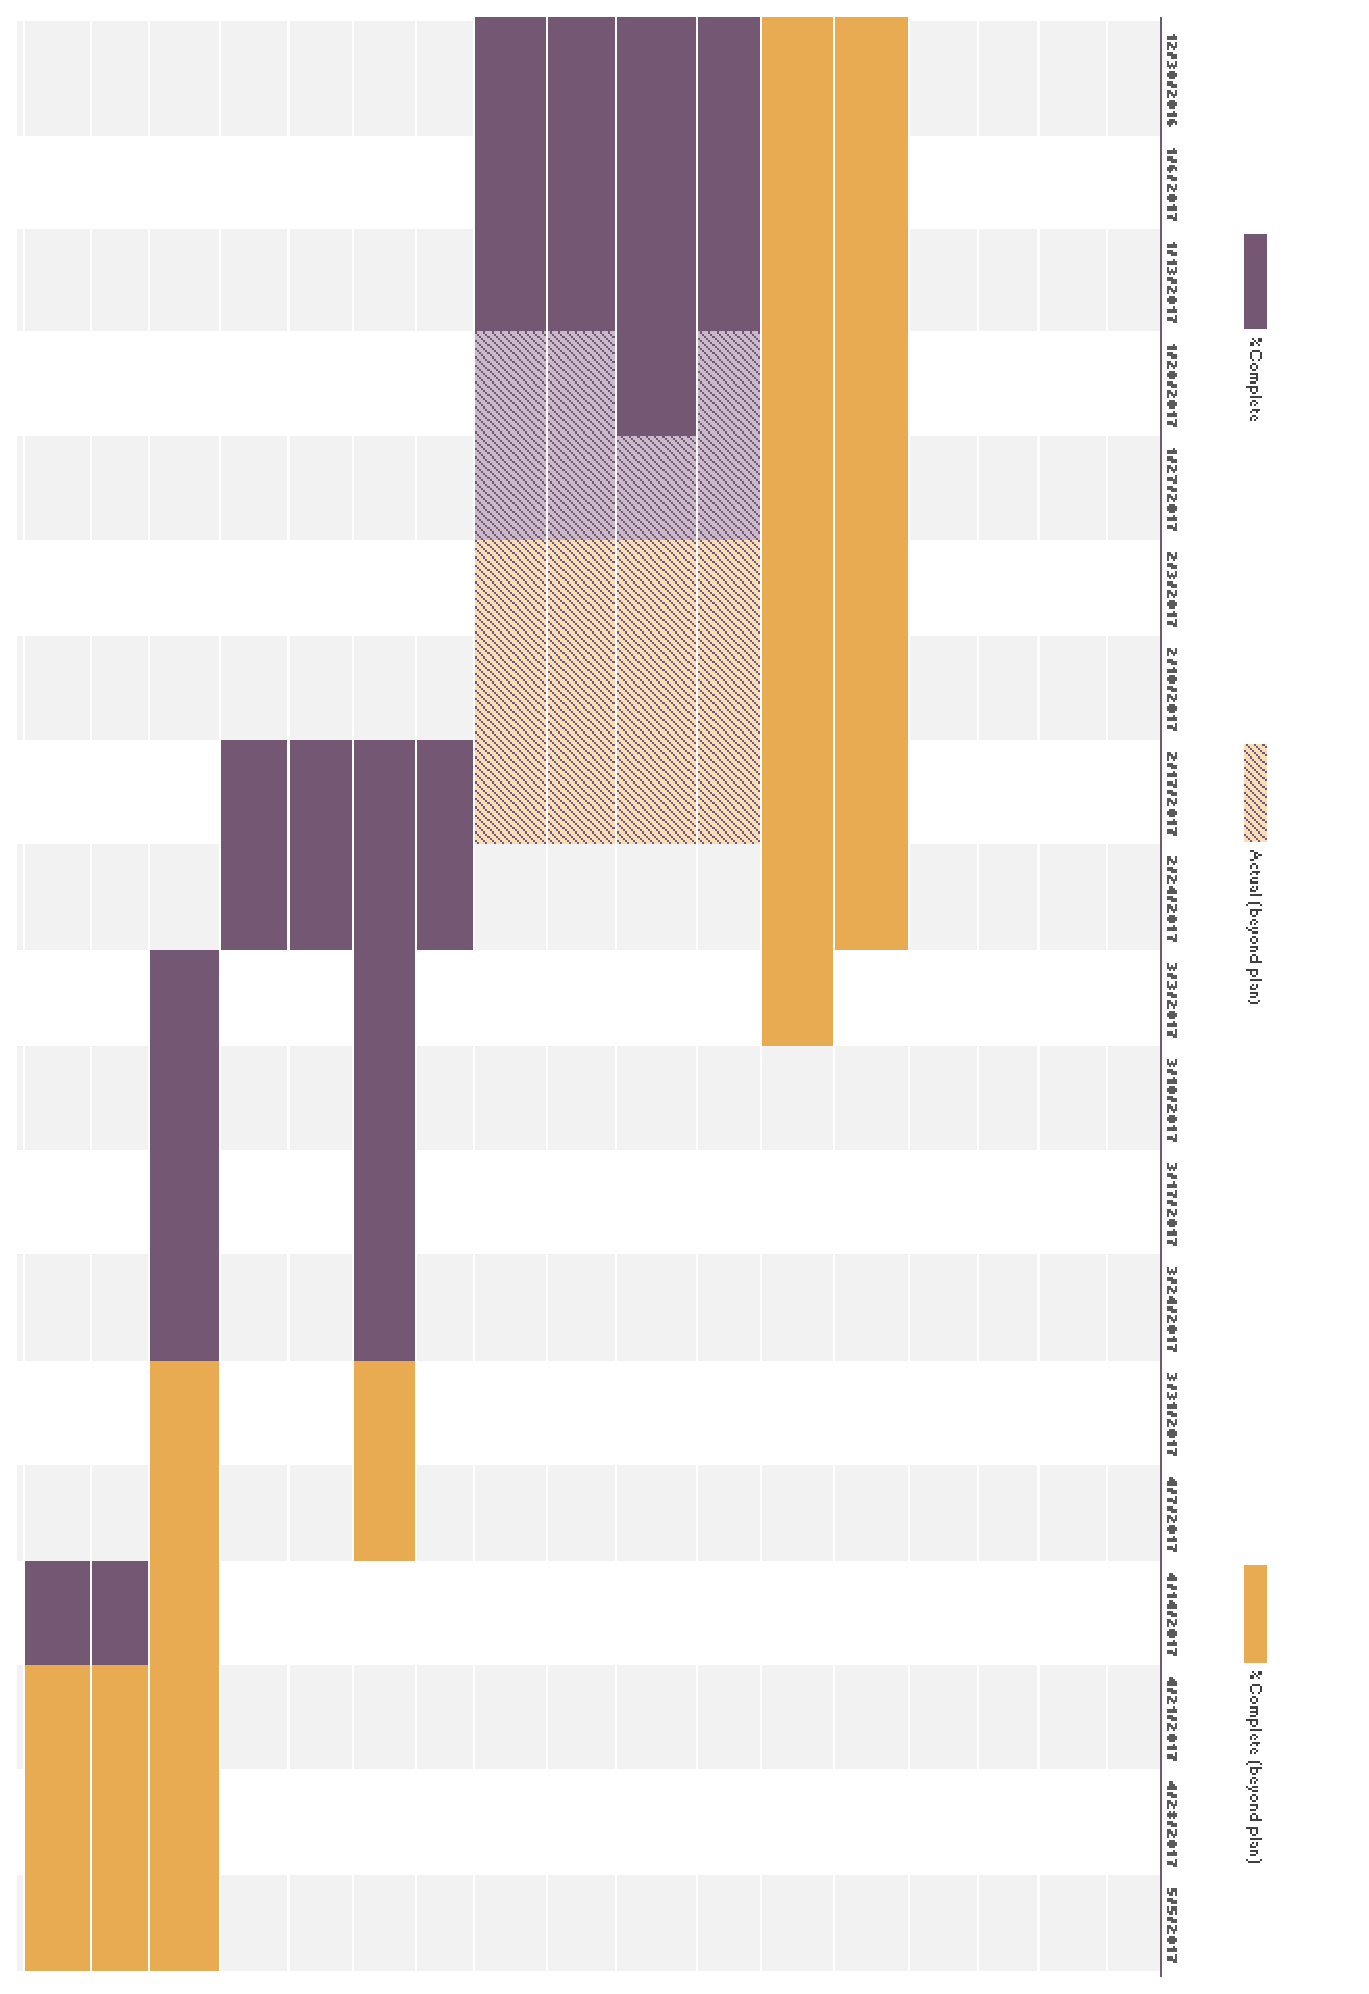
\includegraphics[width=.95\textwidth]{GanttBottom}
	\caption{Bottom half of the Gantt for readability.}
\end{figure}

% Your original design document, as well as a discussion of what had to change over the course the year.
\section{Design Document and Changes}
The original Design Document for this project is inserted in the following pages.

\includepdf[pages={-}]{design.pdf}
\subsection{Discussion of Changes}
The original design of the Visual Studio Code extension was targeted towards web developers.
Discussions with the client transitioned this viewpoint to make the tool more universal and available to a wider audience of developers.
The tool was then redesigned to allow for broader customization through the use of ``grammars'' which users can use to define certain behaviors for the extension.
This change allowed for more customization and tuning available to the user, meaning it didn't really matter what kind of developer they were because they could adapt the tool to their needs.\\

Another change from the original design was the use of certain technologies which will also be discussed below.
The developers had intended to use the programming language Perl and associated libraries to parse the project directories of the user but found keeping the entire project written in TypeScript made more sense and was easier to implement while keeping the same amount of functionality. 
Other technology changes included using a custom implementation of the features provided by jQuery's Advanced News Ticker API library.\\

One major design change from the original document was not parsing the updated file on save or having multiple versions of the parsed data structure around.
It was decided to only parse the project directory when the user explicitly said to (when the user wanted to refresh the file map UI or notification list). \\

It was also briefly mentioned in the original design document that the extension would reformat the user's code.
This feature was removed.

% Your tech review, in its original form. Did you change your mind about any technologies? What had to change?
\section{Technology Review and Changes}
The original Technology Review Document for this project is inserted in the following pages.

\includepdf[pages={-}]{techreview.pdf}
\subsection{Discussion of Changes}
Sam discussed the different parser technologies the project would use to parse the files in the user's project directory.
He started out with the parser class.
It was decided the developers would use a custom parser for the reasons he mentioned in the original Technology Review. \\

The third section Sam talked about was specifically which Perl parsing tool the team would use.
At this point in designing and developing the extension the team was pretty convinced they were going to use Perl as their parsing language.
The design change mentioned above where they transitioned the target audience from web developers to a wider audience of developers moved them away from using Perl.
Perl had a lot of libraries and built in functions specifically to parse HTML which the extension still needed to do, but it was decided it was better to design a more universal parser.\\

Zach then went on to talk about how the extension would store its data.
He mainly talked about different types of databases including SQL and NoSQL databases.
It was decided the team wouldn't use a database at all but rather implement the data structure using a single JSON file which could then be passed to the UI to read to generate the appropriate visualization. \\

As mentioned above in the design changes, the developers decided to not keep two or more versions of the parsed data, so there was no need to have a technology that compared them. \\

Cramer looked at different Integrated Development Environments (IDE) and their respective event listeners and languages they are written in to allow the developers a better experience building the tool for that specific IDE.
The developers decided to use Visual Studio Code for the IDE they would build the extension for.
They did this for the reasons mentioned in the original Technology Review.\\

The team decided to transition to built in events instead of using EventEmitter for the event listeners.
Because the extension is only launched and the directory parsed when the user explicitly tells it to, there was no need for more complicated event listeners than the ones already built in. \\

Eric discussed the different ways to build and show the UI. 
The team decided to use vis.js as the main JavaScript engine for displaying the nodes and edges within the file map UI.
The broken rules (now called notifications) was planned on being displayed using jQuery's Advanced News Ticker API. 
This was overruled by custom code as the News Ticker API didn't add much value in terms of usefulness of the extension.
The actual location of the file map UI was decided to be done within an Electron window.\\

\section{Weekly Blog Posts}
	\subsubsection{Week 3: Cramer Smith}

Week 3 Senior Project Work



This week I worked on the problem statement, and thought about the design of the tool that we are planning to make.



We talked to our client about what he wanted and what he was looking for in our plan. We had some initial confusion about what we were supposed to do. Our client Christopher Scaffidi wants us to use IFT design patterns within a the tool. We were more focused on just making the tool itself. After talking to him we are on the same page. We will be using the tool and make a prototype that we might be able to test by the end of the year. 



Personally I was part of the conversation that about making the design, we are planning on having a code "tagging" system that will allow users to tag their code for the organization mechanism. This is not the final solution but it is the idea we have at the moment, and Chris thinks it's good. I also worked on the proposed solution part of our problem statement. That section still needs some polish, but I was assuming this is a rough draft. I tried to define what types of IFT design patterns we would be using within the tool we are creating and define some parts of IFT. I don't think that I was looking from the 10,000 foot level. I need to work on that in the future.



Thus far the tricky part of our project is that the 'problem' is just to use IFT. That is what our client wants. What we have proposed is not a problem but a solution. We want to implement this tool to prove that IFT within an application makes work easier, or at least test that it does. So that's what we are doing now. 



For week 4



We hope to maybe start working on our requirements, and resumes. I really want to get started on the coding of the project but I think we do that mostly in the winter? Would it be bad to start sooner?  \\ 

 \subsubsection{Week 3: Sam Lichlyter}

Week 3



This week I set up our GitHub page (welcome), I also worked on our problem statement along with the rest of the team. I have been our main contact with our client, Chris, since he and I have worked together for the past year on similar research projects. This week we sat down with Chris to discuss some of the specifics of the project and to form a rough outline of what he wants to see and when.



Earlier in the week we hammered out a few of the main design decisions for our tool and how we expect the user to interact with it, along with what tools we will be using to build ours, and what languages we want to support at first launch.



Next week we plan on getting our requirements document in a near finished state. \\ 

 \subsubsection{Week 3: Zach Schneider}

What We Did This Week

This week was one of logistics and clarification. Sam set up our GitHub repo called Project Postal (a weird name, I know) and each of us made a few initial commits to it. I set up the Latex document for our problem statement, so we will have a .tex template file for future documents. We scheduled the meeting time with our TA, Vee, for Fridays at noon. We won't meet with him this week but will in week 4. We have also be in email contact with Prof. Scaffidi, our project sponsor. He has been clarifying some information for us as we wrote our problem statement. We had some initial confusion as to whether the research aspect of our project was the focus, or if the tool we would be developed would simply use principals of the IFT research. Turns out it's a little bit of both, but I think we all have a clearer understanding at the end of this week. Finally, this Friday we are having our first in-person meeting with Prof. Scaffidi to get the problem statement signed and some expectations established for this project. I may update this post if there is information of note from that meeting.



Plans For Next Week

For the class, we were asked to prepare our resumes to bring in, so I will be updated my existing resume this weekend. Besides that, we have no immediate instructions specifically related to our project. As such, we will do as instructed in class Tuesday. \\ 

 \subsubsection{Week 3: Eric Winkler}

This Week: 

1. The group wrote out the problem statement and spent a little time reworking the abstract. 



2. Began discussing basic design of how Postal will work and made sure that the project was going to be feasible.



3. Just today we sat down with Chris and discussed expectations of the project. It surprised me that we might actually get a chance to run a study with actual people. REUs FTW. 



4. Scheduled the next four weeks. Mostly list what we wanted to have accomplished when and reserved rooms. We're not at the point yet where we're ready to divide up jobs so we'll be working together for the next two weeks at least.





Next Week: 



By the end of the next week we'd like to have our requirements nailed down and start to draft out our design for the system. \\ 

 \subsubsection{Week 4: Cramer Smith}

Week 4



What I did



This week I worked with the team to help define the the problem statement more and start to think about some more basic requirements. I also started looking more at the Visual Studio Code that we are planning to use as the basis of our extension. I was able to easily make a 'hello world' of the extension. And I made my own branch and logged the meeting with a python script that I made it's fun it is working nicely. I need to add some markdown implementation, but I am feeling lazy at the moment. I put it in my HelloWorld Branch.



We met on Wednesday, and worked for three hours hashing out different requirements and the problem statement. 



Our Plan For Next Week



Next week we plan to work on the revision of the problem statement and get that finalized, and go to the career fair. We also plan to go work on the requirements more and I will probably work on expanding the hello world extension. \\ 



 

 \subsubsection{Week 4: Sam Lichlyter}

This week we revised our problem statement. In doing so we focused more on web developers and refined the goals of our product to reflect that. We decided to create a more visual component which we could use to convey the structure of the users code in a more understandable format. 



We also met with our TA, Vee, who gave us some advice on how we should approach the class and our teammates. Being pretty close friends I think we'll be okay and we've had excellent communication in the past, so I'm not too worried about this. 



We started thinking about our requirements and the requirements document which we plan on working this weekend.  \\ 

 \subsubsection{Week 4: Zach Schneider}

What We Did This Week

This week our whole team met to discuss our problem statement revisions and to begin to think about what our requirements might look like. During the course of this meeting, we came to the conclusion that we would be better successful if we pivoted our tool towards two more specific categories: web developers and/or inexperienced developers. Previously we had aimed to tackle large scale projects with experienced developers, but we believe this would have been a problem for us time-wise and knowledge-wise. Additionally, it will be easier to test our tool with inexperienced developers (students) than more seasoned developers. We sent an email off to our client to notify him of our pivot (the details still meet all of his original requirements) and we hope and expect that he will approve them.



The team also meet with our TA, Vee, for the first time this week. We all became acquainted and he informed us of what he expects from us. The meeting went well and he believed our project and team were all currently in a good spot.



Plans For Next Week

Next week we will finalize our problem statement and have it signed. The revisions will revolve around rewriting some of the specific terms to be in accordance with our pivot this last week, as well as adding citations to a source we had used for information. We will also begin and finish work on our requirements document, in accordance with the guidelines specified on the class website. \\ 

 \subsubsection{Week 4: Eric Winkler}

This Week:

This week we spent a chunk of time revisiting our problem statement and started a plan for the rest of the term. We set up a schedule for team meetings which will be weekly. We also spent a good chunk of time discussing basic requirements and touched on the design of our tool. We were mostly attempting to reassure ourselves that our project was feasible and made sense. The result of the discussion was a narrowing of our project's scope.



Next Week:

We're planning on having a completed(ish) version of our requirements done by the end of next week. Additionally we may spend a bit more time familiarizing ourselves with visual studio code its extension system. \\ 

 \subsubsection{Week 5: Cramer Smith}

What We Did This Week 



This week we worked on our problem statement final version. We only needed to add citation so it wasn't that bad. We also made some progress on our first HelloWorld Extension and making it look at the current files for the user. We also started our requirement document.



Our Plan for Next Week



Next we plan to do more of our requirements document and make a lot more progress on our simple prototype.  \\ 

 \subsubsection{Week 5: Sam Lichlyter}

This week we primarily worked on revising our Problem Statement as well as the rough draft of our Requirements Document. We came up with a tentative schedule for what we wanted to accomplish and when. Because we weren't given much direction in class as far as when certain documents are due, we had to more or less make it up ourselves. The schedule we came up with I think will allow us to move forward at a steady pace accomplishing the tasks and getting a working product by the end of Winter Term. This will give us plenty of time in the Spring to test our product with other people.



Next week we plan on getting some functionality built into our extension for VSCode. \\ 

 \subsubsection{Week 5: Zach Schneider}

What We Did This Week

This week the team completed the final version of our problem stated. We added a citations, subject headings, and revised a few lines concerning how we will test our software tool. We also began work on our requirements document. A rough draft has been submitted as of Friday, with the majority of the required sections within the document completed. We still need to nail down some specifics regarding the actual functions within our tool, as well as the operations the user will perform within our tool. 



We met with Vee this week and simply checked in our progress with him. There was nothing specific we needed to do coming away from that meeting, other than making general progress on our documents.



Plans For Next Week

We will continue to iterate through versions of our requirements document, completing and signing the final version by Friday 11/4. We will meet as a team to discuss the details still needed, and we will await and address and corrections as noted by the professors for this class. \\ 

 

 \subsubsection{Week 5: Eric Winkler}

This week the majority of our time was spent writing the requirements document. Part of that process involved getting a very, very rough schedule for our project. We had to mostly make guesses as to how long each component would take but we left some flexibility room at the end. We also made some finishing touches to our problem statement. 



The plan next week is to begin preparing for our next meeting with out client. He'd like to see something on the screen (even hello world as a VSC extension). We're planning on getting our windows set up. \\ 

 \subsubsection{Week 6: Cramer Smith}

What We Did This Week



This week we worked on the Requirements document. While doing this we were forced to make a lot of decisions about the project that we have been needing to make. We were faced with a lot of requirements that we had to define that were previously undefined. I hope that we haven't set ourselves up for failure. 



What We Plan To Do Next Week



With the next week we hope to get a small prototype done for our client, to prove that we have made progress in the development side. We also want to get some paper prototyping done so that we can get a better idea of what we want the application to look like. We also need to do the tech document. I think that is what it is called. \\ 

 

 \subsubsection{Week 6: Sam Lichlyter}

This week we finalized our requirements document. We met up a few times to finish the sections we hadn't finished last week and to revise the ones we had. Cramer and I worked on getting our hello world example to work with VSCode as well as resolve some issues Zach and Eric were having with GitHub and Windows path names being too long. We also met with our TA, Vee, to go over our progress. He also explained what a tech review was to us.



Next week we have another meeting with Chris. We plan on having a few paper prototypes (or derivatives thereof) to show him as well as our hello world extension. \\ 

 \subsubsection{Week 6: Zach Schneider}

What We Did This Week

Our team continued to work on finishing our requirements document this week. We met twice to complete the remaining sections we had not finished by last Friday, then went through and revised ambiguous language and poor grammar. Sam and Cramer also continued to fiddle with our "hello world" extension in visual studio code. This test extension will likely transition into our proof of concept code that Chris asked for by mid November. Finally, we met with Ve to check our requirements progress with him and get some information about the tech review document that we will write next week.



Plans For Next Week

According to the CS461 schedule, we will begin writing our tech review document next week. This appears to be both an individual and team document. As we clarify what technology we plan to use, we will also begin to seriously work on our proof on concept visualization extension. We hope to have this p-o-c complete in two weeks. \\ 

 \subsubsection{Week 6: Eric Winkler}

This week we worked towards finishing our requirements document. We also spent more time discussing design options and what facets of this project were feasible with the limited time we have to implement before spring testing. We also discussed and began work on a prototype for our client that will need to be complete next week.



Next week we will be working on the above mentioned prototype and sitting down with our client to discuss the project's  progress. \\ 

 \subsubsection{Week 7: Cramer Smith}

What We Did



This week we focused on getting out a very simple first prototype for our client. We made a extension that displays all the files in the users work station. We also worked on splitting up the project into 4 main parts that each of us can 'specialize' in. We plan on working on these different parts and each of us splitting them up even more while writing the tech document. 



The four parts are:

  Graphic User Interphase

  Files

  Parser

  Integrated Development Environment



We are still trying to figure out who is going to be a in charge of which part except Sam is probably going to use the parser.



What We Are Going To Do



The next week we are going to get our Tech document assignment done, do some research into other tools that might possibly be better for our project. \\ 

 \subsubsection{Week 7: Sam Lichlyter}

This week I helped to create our "Hello World" extension in Visual Studio Code that would parse the directory in which the user was currently working and create an HTML document that listed all the files in their working directory. Our team also figured out how to take that HTML document and display it inline in the editor. We started working on it using JavaScript but we ultimately decided to go with TypeScript, which is Microsofts version of JavaScript, because almost all the examples of extensions used it. In the next few days we plan on finishing up our Technology Review. We have mostly been working in Visual Studio Code and JavaScript, but I think we should explore other options including other text editors such as Atom or Brackets. They are both similarly open sourced text editors. \\ 

 \subsubsection{Week 7: Zach Schneider}

What We Did This Week

Each team member worked towards producing an initial prototype extension for VS Code to display all subfolders and files in a project directory. This "Hello World" example was shown to our client during a meeting with him Thursday. Chris seemed satisfied with our progress so far, but also gave a few suggestions as to what direction each team member should take going forward. My primary responsibility for now will be to research and start developing a method to serialize and store parsed project file data within some kind of database. This will make it so our project parser does not have to re-parse the entire code project every time a file is changed. This research goes hand in hand with the technology review document we started this week. Each member has divided up various areas of interest/technologies to research and report on for use in our project. We expect to finish this document over the weekend. 



Plans For Next Week

Aside from finishing the tech review document, we will begin to take a hard look at the overall design of our extension. We will continue to meet and prototype as a team to get a better idea of how we want to implement various features, and will compile these decisions in our design document that is due finals week. \\ 

 \subsubsection{Week 7: Eric Winkler}

This week we spent a lot of time discussing design and prototyping. 

We started to really nail down the design of our 'file map'. Ideally, it will look like a big web of files that we can zoom into but should the zooming prove too difficult, we also have an alternate design set up. We're a little worried the file map might be overwhelming in terms of information being displayed to the user but otherwise we're happy with the direction we're planning to take.



Additionally, we spent a good chunk of time prototyping a visual studio code in preparation for a meeting we had on Thursday. We built an application that basically parsed for all the files in the current directory and returned it as html within a separate column in vs code. This got us over A LOT of technical humps we we're worried with.



Our meeting with Chris went well. He gave us a pretty elegant architecture to set up our extension with which naturally divided into four big tasks we could each take responsibility for.



gg \\ 

 \subsubsection{Week 8: Cramer Smith}

What We Did This Week



We spent a lot of time working on the tech document. I specifically worked on the sections:

 IDE: looked at the Brackets, Atom, and VSCode

 Language: looked at TypeScript and Javascript

 Event Handling: looked at htmlpreview, event emitters, and the built in events.

I learned a lot about Visual Studio Code which was really nice I feel like I don't know a lot about VSCode.



What we plan on doing next week

We plan to start our design doc ASAP, and work a little more on our prototypes. \\ 

 

 \subsubsection{Week 8: Sam Lichlyter}

This week we finished up our Tech Review document and figured out a lot of the technologies we will be using throughout our project. The main piece I will be in charge of for our product is the file parser. I learned through our tech review that using regular expressions, which was my original plan, probably won't be enough to parse through real world HTML code. For this reason I have decided we will need to write a Perl script and use some of the already built HTML parser modules to find the tags that we want to check for. One of the Perl parsers will also allow us to check against the W3C standards so we can flag the users code for where they essentially "broke the rules." This module will also allow us to turn it off and check against how most browsers actually render the code since how the browser renders the markup and how the W3C specifies it should be rendered are sometimes different. \\ 

 \subsubsection{Week 8: Zach Schneider}

What We Did This Week

This week the team spent most of our time researching technologies and writing the tech review document. Due to some questions that were brought up from some of our research, we request a one day extension for the document, as we wanted to discuss them before submitting our final conclusions. My role in the document was related to data serialization, as parsed data from our clients' project would need to be stored temporarily in some form. We decided that form would be JSON, and we would use the JSON.stringify function to serialize our parser data. Once the document was complete, we spent the rest of our time laying out the basic framework for our design document.

Plans for Next Week

Next week, we plan to begin writing our design document or our progress report. Due to the short week, we're not sure what work will be completed before the break.  \\ 

 \subsubsection{Week 8: Eric Winkler}

This Week we spent time discussing what our shared data structure will look like moving forward. This data structure will primarily be used by Sam and myself; Sam gathering the data and me using it.



Additionally we spent some time finishing up our tech review. We discussed the options each of use researched and made a few decisions about what technologies we'll be using. As far as I'm aware, we are still sticking with VS code and Typescript as our primary technologies, and using a JSON file for data storage.



Next week we should be doing a bit more prototyping and working on our presentation and poster board. \\ 

 \subsubsection{Week 9: Cramer Smith}

What I did This Week



Not a whole lot. I did look around the documentation for VSCode and started to think about the design document. That is truly what spurred the curiosity to look further into the specific documentation of VSCode. I am worried we won't know enough to write a fully fledged design document. I hope to look into this more during the break and will try to do some programming this week. 



Plan for Next Week



We plan to start and finish the design document, and work a lot on our actua project. I feel as though working on the design document should fuel the work on the actual program.   \\ 

 \subsubsection{Week 9: Sam Lichlyter}

This week being a long holiday weekend I didn't work on a whole lot beforehand. I do plan on looking over everything we need for the parser and how to build one. Also at a more basic level I plan on looking over some Perl tutorials to get a better handle on the language. 



Next week we plan on working on our Design Document and finishing it up as well as another meeting with our client.  \\ 

 \subsubsection{Week 9: Zach Schneider}

What We Did This Week

This week the team discussed our schedule for completing the design document, the progress report, and what work we want to accomplish on our extension for the rest of the term. I also researched options for the visual portion of our progress report--I opted for OBS and PowerPoint as I am most familiar with those tools. Aside from this, nothing else was done due to the short week.

Plans For Next Week

Next week we will begin writing our design document. We will continue work on the prototype extension with the goal of having another feature done before our meeting with our client on Friday. \\ 

 \subsubsection{Week 9: Eric Winkler}

This week we haven't yet committed much time to the project. The plan is to begin work on a first version of the file map within the next couple of days. The goals of this first version will be to read in test data from a build of our current shared data structure and render them as objects with Visual Studio code. We are planning on starting off with vis.js and moving through our other options until we find something that will work within the VS code environment. \\ 

 \subsubsection{Week 10: Cramer Smith}

What we did this week 



This week we made a design document. This made us look more into the details of our project and 'how' it was going to work. We also met with our client and showed him our most recent prototype. I feel like he was not happy. 



What we plan todo next week



nothing have a nice break during finals, then during break we will work on getting the prototype working way better. \\ 

 \subsubsection{Week 10: Sam Lichlyter}

This week we finished up our Design Document. We also had a meeting with our client in which we talked about the progress we made since our last meeting as well as our plan for what we want to get done over the Christmas break. I also messed with our parser a bit make it better at finding what we wanted. \\ 

 \subsubsection{Week 10: Zach Schneider}

What We Did This Week

The entirety of this week was spent completing the design document. We all met earlier in the week to define what each team member would write about. We each tackled the general scope of the components we discussed in our Tech Review last week. I covered the data handling portion, that is, the data structure, serialization of the data, and storage of the data into a JSON file. These components were introduced and discussed in light of their respective design viewpoints, according to the IEEE 1016-2009 document. Additionally, we met with our client Chris to discuss the progress we've made thus far, as well as our plan over winter break.



Plans For Next Week

During finals week, we plan to write our progress reports for the term and create a verbal presentation of those reports. We are confident that the report will be thoroughly completed by the due date on Wednesday. Post finals week, we will continue to work on our VS Code extension over the break, and plan to have a rough prototype with parsing and UI completed by the beginning of Winter term. \\ 

 \subsubsection{Week 10: Eric Winkler}

This week we primarily worked on building out our design document. This was a lot hard than the previous documents as we had a bit of trouble trying to interpreter the IEEE standard. It was fairly vague in it's explanations. We later found out during our TA meeting that that was by design as a highly specific document might place constraints on a projects design. We also had a brief meeting with our client to discuss plans and deadlines for over break.



Next week we will be primarily working on our final report for the term and making plans for the next few weeks. \\ 

 \subsubsection{Week 1: Cramer Smith}

What We Did



This week we met with our Client and showed him our first prototype. It was not to the point that we wanted but he seemed very happy with the results and gave us some good feedback and advice for the future. 



We did a lot of work toward getting our extension into an actual working product. Previously we had three different parts and now they are finally coming together. But the bring these parts together was more work than we initially thought it would be. There was a lot of debugging and a lot of frustration, but we are quickly getting much closer to our end goal.



What We Plan to Do



This next week we are going to crank it down a notch. We don't have a deadline from our client until the end of february and we should be able to work more slow and steady rather than this weeks full pace non stop. But we will keep working on it. \\ 

 \subsubsection{Week 1: Sam Lichlyter}

Winter Break

Over winter break we tried to get a lot of the development done while we had some extra free time. The UI logic that Eric was working on is pretty close to being finished, I worked a bit on the parsers over break but didn't make a ton of headway until this week actually. 



This Week

Like I said, this week I made significant progress on the parsers. I worked mainly on getting data from each of the files we were parsing and Zach and Cramer worked on taking the data I had found and serializing it into a JSON data structure that our UI could read. Before we had pretty separate pieces all doing different things, but this week we put them all together so they could all communicate which tied up our project pretty nicely. 



We also met with our client this week to catch up on our progress over the break and decided where we would go from here.



Moving Forward

Looking to the rest of the term we still have a few feature we need to implement like getting the links between our nodes to show up, I know we're actually really close on this. Our client gave us some pretty good advice about hooking up our parser logic to the UI and how our users should interact with our tool. We also talked about timelines and what milestones we should aim for within the next couple of months. \\ 

 \subsubsection{Week 1: Zach Schneider}

What We Did Over Break and Week 1:

As of this week, our team is in a pretty good spot concerning work we've done so far and goals we're working on currently and in the future. Sam, Eric and I are all from the same town so we were able to meet up briefly at the beginning of break to determine what we wanted to accomplish. We essentially decided that we wanted each separate piece of our project to basically be in a working prototype state by the end of Week 1 of Winter Term. Each member of our team had previously undertaken a general concern/category within the project. We informed our other team member, Cramer, of our plans following the meeting. We then each made separate progress over the rest of the break. The UI, the data layer/transfer, and the file parser reached a working state during this time period.



The team had scheduled a meeting with Chris Scaffidi (our client) for the end of Week 1, and our general hope was that we could have some of our project pieces complete and put together by that time. Unfortunately, the "assembly" process was much more time consuming than we initially anticipated, even after working a couple dozen hours between us during Week 1. Despite this, Chris was fairly happy with our progress so far and believed we were on track both time-wise and feature-wise. His goal for us was to have a prototype that we would be able to use by the end of February, and a prototype that other CS friends could use by the end of March. We believe these timelines align with Kevin's "alpha" and "beta" dates set on the course website.



Plans For This Week:

This week, we continue to make progress on each respective feature or function that seems the most relatively crucial to the project. I'm continuing to flesh out the parser->UI data layer so that more parser data can be transferred. We're in a spot where the whole team can work together towards commons goals, rather than individual ones as before break. \\ 

 \subsubsection{Week 1: Eric Winkler}

Over break, the Postal team began implementation. We had three primary modules that were worked on be different people. Sam worked primarily on the parser, Zach on the JSON implmentation and access methods and myself on the UI.



Over break I created the UI within an electron application. The UI is currently capable of reading in our standardized JSON and generating an interactive file map. The file map nodes are color coded by file type, have a size determined by the number of links to the node, can be dragged around and feature a mostly complete implementation of the "dig down" functionality. The file map can also be zoomed and panned.



The next step is to update the file map to be generated on a command from VSCode. We're currently having a little trouble with this as it appears that electron needs to be launched in a certain way from its own process.



WE also had a meeting with our client this first week. We brought him up to speed with where the project is and what was giving the team difficulty. He offered some very good advice about how to further develop the tool. He specifically said to focus on the one feature that makes our tool most useful and to think about what situation it might be most beneficial for testing purposes. \\ 

 \subsubsection{Week 2: Cramer Smith}

What we did this week



This week we met and talked out some of the progress we are having. We also assigned some more work to me.



What we are planning to do



In the next week I hope to work on the Error handling and the UI that the user will see. \\ 

 \subsubsection{Week 2: Sam Lichlyter}

This week

This week we met up to go over the progress we'd made since last week. Eric made some progress on the UI, Cramer made some progress on getting the editor to show the errors we find, Zach and I worked on the parser a bit to get our links working that didn't work last week. Zach and I are pretty close are getting the links to work as well as passing more data to the UI.



Next Week

Next week I would like to get the UI to display nodes for directories we find in the main directory we're parsing.  \\ 

 \subsubsection{Week 2: Zach Schneider}

What We Did This Week:

This week the team met to see where our project stood, what functioned and what needed to function next. Eric continued to make progress on the Electron UI which displays each file in the project, while I continue to work on created the links between those files. By the end of the week, links between files were displayed visually in the electron UI. However, there most likely will need to be a rework of this functionality: the links are generated independently of the project files, which causes major id number incongruities for larger web project when parsed.



Plans For Next Week:

Going into the next week, I will work on reworking the link generation system in the parser. This may or may not be a large effort, but it may go more smoothly if I work with Sam to get the file data I need from the parser. Meanwhile, Cramer and Eric are starting to working on triggering the parser by a save operation within VS Code. Eric will have the UI update accordingly at the same time as the save action. \\ 

 \subsubsection{Week 2: Eric Winkler}

This week we met to discuss some bugs with the extension when it parsed larger projects. The leading theory was that the parser would create a JSON that had links to node ids that didn't have their own structure in the JSON. This caused the GUI to try to link nodes that might not have existed. Otherwise, the extensions performance seems to work well on larger (+100 nodes) projects so far.



The plan for the weekend is to get the "dig down" functionality refactored. I'll probably be adding a couple buttons to help control that. \\ 

 \subsubsection{Week 3: Cramer Smith}

what I did this week



This week I didn't really do too much. I started working on my error handling. It doesnt quite work but it does highlight a line all red.



what I plan to do next week 



This next week I hope to get it fully working and start work on my error UI. And figure out how to trigger the extension on save. \\ 

 \subsubsection{Week 3: Sam Lichlyter}

This week

This week I didn't get as much done as I was planning. I made some progress on the parser but didn't get to working on the links or getting the directories to show up as nodes. Our team also met up and decided we should move our creation of the data structure to the parser instead of parsing then creating the data structure. This would save some overhead of passing data around and would prevent us from touching the data twice.



This will be my task for next week. We also met with Vee for the first time this term to catch up and go over what we would be doing this term for the class, apart from working on our project. \\ 

 \subsubsection{Week 3: Zach Schneider}

What We Did This Week

This week was a relatively slow week for most of the team. We met with Vee on Monday to discuss where we were on our progress and then met as a team afterward to see where each member was on their individual tasks. We are all content with the progress we've made so far, but all agree that February will require a bit more work time put in. We still aim to have a fully functional prototype by the end of February.



Plans For Next Week

Next week should see significantly more work done, as we're all pretty busy with other concerns this week and on the weekend. I plan to rework the creation of file nodes so that links will be correctly supported for Eric's UI, and I will work with Sam and the file parser to ensure this is done sustainably. \\ 

 \subsubsection{Week 3: Eric Winkler}

This week I mostly focused on getting our electron/node GUI to launch when it is called from the vs code extension. It's not quite working yet, but I believe I'm getting close. I've been looking into a node module called process-bridge which should help out with this problem.



I hope to be done with this next week and also start on the dig down refactor and styling the window. \\ 

 \subsubsection{Week 4: Cramer Smith}

I worked on the error notification system



I plan on working on the on save event, and continued development on the error UI. \\ 

 \subsubsection{Week 4: Sam Lichlyter}

This week

This week I got a little more time to work on the parser than last week, but I still didn't get the directories to show up. I think I will hand this off to Zach because he seems to be working more with this data than I am at the moment. I'm going to move on for now and switch our program to a more defined Model View Controller design pattern. Eric has started creating a controller, I just need to refactor the code we wrote for the VSCode extension itself. 



Next Week

Moving our extension to MVC might take a little longer, so I will also work on this next week.  \\ 

 \subsubsection{Week 4: Zach Schneider}

What We Did This Week

This week the team met up and made some progress on each of the pieces we've tasked each other with going forward. Eric successfully launched our Electron UI window from the extension itself instead of the command line, serving as a major step forward for the UI. I continue to rework the Data Structure file node generation, which is conceptually proving more difficult than expected. I will work with Sam going forward to make sure the parser gives me the data I need. Cramer successfully got code highlighting working, a step in the right direction for our error management. We also had class this week which informed us of our upcoming progress report and OneNote tasks.



Plans For Next Week

I will set up OneNote for our "Engineering Notebook" and begin to compile the information we need to make our midterm progress report. I will also continue working on fixing Data Structure file node generation. \\ 

 \subsubsection{Week 4: Eric Winkler}

This week I finally got the GUI to launch from the extension pragmatically! this took quite a bit longer than I thought it would (it shold not have been this hard...) I didn't actually need to use the process bridge to get it to launch. Instead I found the electron has an executable buried way, way down in its npm package directory. I can launch that from a new node thread and everything seems to work. It also works on the three OSs we're concerned about. 



The process bridge wasn't a loss as we'll probably need it for communications between the two node processes. \\ 

 \subsubsection{Week 5: Cramer Smith}

What I did this Week.



I made a function that does a regex function over a file line by line



What I plan to do next week



The next week I plan to work on the details of getting our extension on the 'store' and getting it out to the people.  \\ 

 \subsubsection{Week 5: Sam Lichlyter}

This Week

I started to move our extension to an MVC framework. To do this I basically took a lot of the functionality we had and "functionalized" our code into a controller class. This will also help Zach out with his asynchronous issues he's having so he can just call one of these functions when he needs to instead of having to other workarounds.



Next week

Next week I will continue moving things over to MVC.  \\ 

 \subsubsection{Week 5: Zach Schneider}

What We Did This Week

This week I began to wrap up node creation in the data structure portion of our project. The display of href links between nodes has continued to be tricky, and isn't fully featured or functional yet, but I believe this can be added to over time. The rest of the team worked on their respective portions as well.



Plans for Next Week

Once we are in a good place concerning the actual project, the team will convene to work on revising the tech review and design document. Tech review should be short and sweet, while the design doc may take some serious reevaluation. Kevin allowed us an extension for our progress report in light of our attempt at a beta release by Week 7 instead of 11. The progress report will be completed by the end of Week 7 instead. \\ 

 \subsubsection{Week 5: Eric Winkler}

We spent this last week developing and working towards a plan to provide a public release of Postal on the extension marketplace. This release will not be entirely feature complete but we'd like to have feedback on what we currently have working by the end of the month. Our plan is to finish all functionality short of errors, release what we have on Monday (2/20) and during that week finish errors and solicit feed back from both the market place and personal connections. 



I will be focusing on cleaning up the UI and getting the nodes in a hierarchy arrangement. We came to the conclusion that displacing both links in terms of includes and hyperlinks as well as displaying links that indicate a node's position in the project directory was overwhelming. This is especially true in a web like configuration of nodes. Instead, we will display the nodes in a directory based hierarchy where the links displayed by default will be indicative of the node's position in the project directory. When a node is clicked on, the links that indicate a connect between files (includes/hyperlinks) will then be rendered. \\ 

 \subsubsection{Week 6: Cramer Smith}

What we did this week



This week we went over our old documentation and I made a line by line parser that we now don't need. That's ok.



What we plan to do next week



In the next week we plan to get our 1.0.0 out, and then we will make video of our mid way point.  \\ 

 \subsubsection{Week 6: Sam Lichlyter}

This Week

This week we updated a lot of our documents as per requested by Kevin including the Tech Review and the Design Document. This was good because enough had changed in our design that our old design document was out of date. This weekend, we sat down and refactored our entire extension. It is now more reliable and actually has more features than it had before we started this weekend. 



Next Week

Next week we will work on our Progress Report because it was extended a week by Kevin for us because we wanted to get our extension on the VSCode Extension Marketplace as soon as possible. We will also work on uploading our extension to the marketplace and finishing up the refactors by tomorrow evening. \\ 

 \subsubsection{Week 6: Zach Schneider}

What We Did This Week

This week the team spent most of our time working on revising our various documents. Minor revisions were made to update our design document, while some serious portions of the tech review had to be updated. I was in charge of setting up the One Note pages and formatting them correctly with all the needed content for our midterm progress report. Lastly, we scheduled a team code review for this weekend so each member can understand what everyone else is working on. Hopefully this leads to cleaner and more functional code overall. We plan to work a lot this weekend in order to reach our Beta release by next week so we can begin user testing.



Plans For Next Week

Next week we will finish our progress report presentation, as we received an extension on it. The extension is due to our accelerated work timeline for our actual project. If all major features are completed by the end of the week, we will begin working on implementing error identification and visualization for our user's projects. \\ 

 \subsubsection{Week 6: Eric Winkler}

This week we began the process of of refactoring all of postal. It actually turned into a complete redesign and rebuild from scratch. I mostly headed the redesign while Sam became our Code-driver. As a result there are now clear Interfaces between our Parser, Controller and UI and all of our code is of a much higher quality. I will be doing a design document update to reflect these changes, they are a little too numerous to mention in a blog post. At a high level the extension now works like this:

The user luanches the Postal extension.

Our extension calls our controller which then:

   Finds all files and directories recursively.

   Calls the parser to parse each file. This returns an array of standardized Tokens.

   The controller turns those tokens into our JSON File and calls the UI.

   The UI reads the JSON and launches. \\ 

 

 \subsubsection{Week 7: Cramer Smith}

what we did This week 



This week we completely redid the extension. We made a lot of improvements to the prose and the th way that the graph is generated in the UI. I dont know how it works but it seems to work really well

We also put the extension up on the market place. This is great cause now we can distribute our extension much easier.



what we plan to do this week 



I would like to get a some settings done for our extension. done w \\ 

 \subsubsection{Week 7: Sam Lichlyter}

This Week

This week we continued to work on our extension. The biggest thing was we uploaded it to the Microsoft Visual Studio Code Marketplace so we could get users feedback on it. So far we haven't heard from any users on the store but we have given it to a few of our friends to test it out for us. We fixed some bugs related to the store and some general ones we didn't realize were there until we gave it to people. 



We also put together our progress report this week.



Next Week

Next week we have a meeting with our client and we also plan on pushing some more bug fixes to the store. \\ 

 \subsubsection{Week 7: Zach Schneider}

What We Did This Week

This last week was extremely busy. The team worked all weekend, essentially re-writing each component of our project, piece by piece so that they would support the required design specifications. Previously we had had a mostly working prototype, but could not build on it any further. The parser saw the most work re done, followed by the UI then the data layer. Ultimately, we achieved the milestone we wanted and published our extension to the VS Code extension marketplace, where users can now download and use it. Additionally, we completed our progress report, which we had received an extension on last week.



Plans For Next Week

Next week we will meet with our client, Prof Scaffidi to show him our progress and find out about the research component of this project. We will continue to test, bug fix and add features to the extension, particularly around error detection in a user's code. We also have class next week to learn about how to present our project at Expo. \\ 

 \subsubsection{Week 7: Eric Winkler}

This week we finished our refactor of Postal and implemented a few new features (our dig down is currently working better than before). We also published it on the store on Monday and have been bug fixing since. We still have to implement the one click links appearing and error parsing. 



A challenge we have is that our npm modules are too big to include packaged in our extension, so we have to currently have the user run 'npm install' in their extension directory before it will work. This is not ideal and we're currently looking for ways around this. \\ 

 \subsubsection{Week 8: Cramer Smith}

What I Did This Week



Well we met with chris. Was that this week? Yeah it was, and he wasn't as happy as we had hoped. I did get a simple start on setting though and I am happy about that, I don't know if we will use them.



What I plan On Doing This Week



This week we plan on making the extension more useful. We have a huge list of features that we plan to add this weekend. \\ 

 \subsubsection{Week 8: Sam Lichlyter}

This Week



This week we met with our client to show him our progress on our extension. He gave us some valuable feedback on the UI of our extension. We went on to try and implement these as well as fix some of the bugs we found last week.



Next Week



Next week we plan on getting c-like functions going. \\ 

 \subsubsection{Week 8: Zach Schneider}

What We Did This Week

We started the week of by meeting with or client, Chris Scaffidi. While he was happy about our progress, he still felt our project/UI wasn't to the stage of usefulness yet where someone (or us) would want to use it every day. So, our goal going forward is to move from the core visualization functionality, to making that visualization useful. This will include letting users jump to the point in code that each node represent and better visibility with node names and relationship. We will convene again this weekend to hash out much of the work that needs to be done.



Plans for Next Week

We will evaluate where the project is after our work/code review this weekend. We hope to solidify the rest of the core functionality of the parser and begin adding "gold plating" features (though at this point those features are more or less necessary). Our new major deadline is the end of the term when we hope to have our project in a "useful" state. \\ 

 \subsubsection{Week 8: Eric Winkler}

This week we met with our client and decided on a list of features to complete in the next couple weeks. this includes refactoring our UI with a new vis method called clustering. Additionally we will be implementing C-like function parsing and  other UI features like being able to switch between web view and a hierarchy view. \\ 

 \subsubsection{Week 9: Cramer Smith}

What we did this week.



Almost nothing. We worked some this weekend we now have C functions working. That makes our parser way more useful to me personally. 



What we plan to do next week



Next week there are a number of things that we need to do. We have to do our progress report again and make a video thing for that. We also hope to have our project entirely done by the end of this quarter so we will probably work on the final touches of our extension and get it up on the marketplace and see if we can get some actual users.  \\ 

 \subsubsection{Week 9: Sam Lichlyter}

This Week



This week we implemented c-like functions. This allows our tool to visualize c-like functions similar to the way we visualize divs and links in our web projects. We also tried to implement a character-by-character parser, but we decided we could rework our current parser to parse the whole file at once and still get the same features we wanted out of a character-by-character parser. We also started on clustering our nodes.



Next Week



Next week we plan on getting our clustering to completely work as well as some other basic features like navigating to the users code when they click on links, not parsing the user's comments, and getting a .postalignore working so they can specify which files they don't want our extension to parse.  \\ 

 \subsubsection{Week 9: Zach Schneider}

What We Did This Week

This week each team member spent most of their time on individual work on adding features to the project. I worked on adding configuration buttons to the UI that allow the user to dynamically change the shape and physics of our information network. Later, I began working on the UI for the list of errors that our parsers will detect in each file. Lastly, the team began making preparations for our progress report video and preliminary poster due next week.



Plans For Next Week

Next week we will meet to put together the basic version of our Expo poster, deciding what points we want to hit and how we want to display our UI. Additionally, we will continue adding minor features to our project, such as the error list. \\ 

 \subsubsection{Week 9: Eric Winkler}

This week we planned on implementing a character by character parser but instead opted for a sort of priority base parser that reads in the entire file. This allow us to write grammars for things that may appear on multiple lines like for c-function definitions. Additionally we began the process of switching over to a clustering method for our UI nodes and Zach worked on UI controls. \\ 

 \subsubsection{Week 10: Cramer Smith}

What We Did



We continued work on the large todo list that we feel we need to have finished by the time of actual release, and we are making progress. I specifically working on the process bridge that will connect the electron terminal to the Vscode IDE. 



What We Plan To Do



With Spring break finally here I think some of us are going to take a small break. I myself think I will try to get the process bridge working and have the users be able to navigate to the code from the electron window, but we will see if I will be able to accomplish that. \\ 

 \subsubsection{Week 10: Sam Lichlyter}

This Week

This week I fixed our postalignore to allow a set of files or directories to ignore by the parser. I also moved it the settings that the user can edit within VSCode. This is instead of a separate file they would have to include. I also built a new grammar and parser behavior to allow comments to be ignored. This fixed some issues where `if` and `while` blocks were being considered functions by our default grammars. \\ 

 \subsubsection{Week 10: Zach Schneider}

What We Did This Week

We had two major goals we worked on this week: completing our preliminary Expo poster and finishing a number of UI features for our project. The poster had a bit of a rough start; we all did a part of the poster separately, then later realized that the whole thing was too wordy and not cohesive. We revamped the poster as a team, focusing more on why we did what we did rather than including so many technical details on how we did it. For the project itself, I worked on adding a sidebar window that will display an notifications or errors the parser finds for each node in the main UI. The visual elements are there, it's just down to getting the parser to generate the right data to populate the window.



Plans For Next Week

Next week we will each work on our individual progress reports as well as the team video report. It should be mostly the same as the one we did a few weeks ago for the midterm. We may make minor updates to the codebase as well. \\ 

 \subsubsection{Week 10: Eric Winkler}

This last week we began to implement the last few features for a close to finished version of postal. I worked a bit on fixings some bugs with the new node clustering system. Additionally I added the ability to see link information (line numbers) when links are selected. This was harder to do than I originally anticipated. The clustering system actually creates all new edges and nodes when things become clustered, so finding the correct objects to manipulate was a bit of a pain. Additionally I reintroduced file links as red lines but they will be changed again here relatively quickly.



Next I will be working on adding options for displaying file links, making sure our process bridge is working correctly and adding a couple of UI controls. \\ 

 \subsubsection{Week 1: Cramer Smith}

What We Did Last Week



We had spring break and we all worked somewhat sporadically over the break, not that much though. Then we got back to school and we met on Monday and worked on some bugs and features that needed to be added. We got those to a working stage and then we met with our client on Tuesday. This meeting went poorly. He really wanted progress on the UI and we haven't been focusing on the UI as much as the functionality. That was disappointing, but with what we have set up already we feel we can make the changes he wants to see by our next meeting. So those changes are what we have been working on.



What We Plan To Do 



This next week we meet with our client and hopefully show him a better UI. If that meeting goes well he will start gathering funds for testing and get us started on making good experiments for users. We also will continue to squash the numerous bugs that we are running into with the extension. \\ 

 \subsubsection{Week 1: Sam Lichlyter}

This Week

This week we met with our client who was slightly disappointed in the progress we had made in the last few weeks but offered valuable feedback and a chance for us to try again next week. So this week we have focused primarily on the feedback given to us by our client so we can meet his expectations by our next meeting. I have mostly been in charge of changing some of the subtler UI elements to make the tool more user friends and a bit easier to find/navigate information. \\ 

 \subsubsection{Week 1: Zach Schneider}

What We Did This Week

This week we met with out client to check in with our progress. We had a bit of a misunderstanding of work focus: we had been polishing off features whereas he wanted us to focus on polishing the UI. As such, we will meet again next week to check our progress again. Various features were worked on this week, mostly related to the UI. We created a number of event listeners that allow users to click on our node network and be directed to the corresponding line of code in their project. Additionally, we created a TypeScript grammar that will allow us to visualize our own project, as it is the main coding project we actually all work on day to day.



Plans for Next Week

We will continue polishing the UI to get it up to our client's expectations. We have a meeting with him on Tuesday to see if the work is to his liking. After that, we will see if there is time/resources available to conduct user testing. \\ 

 \subsubsection{Week 1: Eric Winkler}

The week We implemented a few new features and had a meeting with our Client. 

I spent a bit of time working on fixing some performance problems with vis.js. When running in a hierarchical mode, vis runs several optimization algorithms in an attempt to limit white space between nodes. However, our trees aren't perfect and can nodes can have links over several levels of the tree and this seems to cause vis to hang when it tries to optimize. I'm currently midway through trying to massage the input such that vis will begin to behave in a more useful way. 



The result of our client meeting was that we would need to work on the UI a bit\and focus on using the tool daily. We're planning on meeting with him again next week to show our progress.  \\ 

 \subsubsection{Week 2: Cramer Smith}

What We Did This Week



This week we worked on improving the UI for our client. We made it more responsive and improved the quality of information that is produced and shown on the UI. But with all this improvement we also introduced a number of bugs that will need to be addressed in the future. But with the improvements we showed our client we were able to get him satisfied with what we had and he said that we should start organizing a testing group that will try the extension and that we can get results from the tests and maybe publish the work. This meant we had to get certified by the IRB, so we worked on getting certified and working on creating a short questionnaire that we will use to quantify the results of the tests.



What we plan to do this week



This week we hope to address some of the more pressing bugs and create two use cases that the people we will be experimenting on will be using during the test.  \\ 

 \subsubsection{Week 2: Sam Lichlyter}

This Week 

This week we worked on fixing minor bugs within our tool. For example we had some UI that was a little wonky that we fixed up, we also still have a bug that catches if, else, while, etc. blocks as functions when defined in TypeScript. But mostly minor bugs like this were taken care of this week. We also met with our client again to to talk about IRB testing. This went well and we have a plan to move forward in the coming weeks to get testers.



Next Week

Next week we plan on fixing smaller bugs for our tool, but I think mostly our focus will be on the poster board that's coming due soon. \\ 

 \subsubsection{Week 2: Zach Schneider}

What We Did This Week

This week we finished up most of the UI changes we felt Chris cared about most (font, node hierarchy, readable notifications) and demoed it to him on Tuesday. He was satisfied with our progress and began the discussions about user testing. That will be our main focus outside of Expo going forward. We are writing questions to ask the users once they have tested our project that we will submit to the OSU IRB Monday. Additionally, we worked on our Capstone poster second draft. We are planning on capitalizing on the extra credit opportunity concerning the poster board by working with another team.



Plans for Next Week

Next week we will begin creating the tasks the users will perform in our study. We will also continue polishing our project to make sure it's totally ready. We will refer to Chris to make sure our study is sound. \\ 

 \subsubsection{Week 2: Eric Winkler}

This week we continued to adjust postal to better fit our client's needs in anticipation of a meeting we had on Tuesday. He was happy with the improvements we had made and was also pleased that we were using the tool on our own time. We began to make plans for testing and created a new timeline for the group. In the next few days the team will get IRB certified and create a list of questions that will eventually become our end of test questionnaire. I personally will be working on a couple of bugs I noticed as well. \\ 

 \subsubsection{Week 3: Cramer Smith}

What We Did This Week



This week we worked on some minor bugs, we met with Kirsten about our poster, and we started working on getting demo projects for our user testing. This was difficult because we had to make two projects that were similar but not so similar that they had problems that were in the same or recognizable spots. We need the first test to not teach the user information of the second test. The Poster feedback we got was that we need less (more concise) text, and the pictures need to be a bit bigger. There were also some nitpicky changes that we hope to change.



What We Plan To Do Next Week



This week we hope to make all the improvements on the poster and the get some bugs fixes for the extension and finish the demo projects and maybe even get some our friends to unofficial run through our tests and questionnaire to get an idea of how the tests run and how they feel to user and for us as testers, but we will see if we get that far. \\ 

 \subsubsection{Week 3: Sam Lichlyter}

This Week

This week we met with Kirsten to review our poster and another group's poster. We also started working on our user tests for our IRB testing. We also finished all of our IRB certification this week. We didn't really run into any problems other than things we needed to fix on our poster which we just got that feedback today. 



Next Week

Next week we plan on continuing working on our user test. \\ 

 \subsubsection{Week 3: Zach Schneider}

What We Did This Week

This week we submitted our user testing proposal off for IRB approval via Chris. This proposal included the questions we planned to ask our users and our own Human Subject certifications. Additionally, we further tweaked our project to make it completely testing ready. The team discussed the nature of the tasks we will ask users to carry out in order to test our project. These tasks should be finalized by next week. Lastly, we met as a team with Kirsten to receive feedback on our Expo poster and how we can explain our project more clearly.



Plans For Next Week

Next week we will make modifications to our poster according to the feedback we received, then send it off to Chris for final approval before Expo submission. Secondly, we plan to finalize our user testing plans as we wait for IRB approval to come back to us. Lastly, we'll check if there's any word on whether we have to do a midterm progress report again this term. If so, we will start on that. \\ 

 \subsubsection{Week 3: Eric Winkler}

This week the team continued forward with our plans to prepare for testing. Our client has a hold of our certificates for IRB approval and our list of questions. He suggested that we begin prototyping the trials for the test and have a rough draft of the experiment by next Monday. We plan on completing this this weekend. 



I also had a quick meeting with Eugene Zhang looking for feedback on our UI. He has some pretty good ideas as to how to make the UI a bit more intuitive and also put me in contact with Yue Zhang. I will be meeting with her next week to get some feedback on the project as well.



This weekend I also plan on doing a redesign of our poster as a result of a feedback meeting we had today. \\ 

 \subsubsection{Week 4: Cramer Smith}

What We Did This Week.



We had to finish up the bug-crunching and adding the last small features to our extension in expectation of the code freeze. That approaching this coming up on Monday. The major requirements that we had to complete were:



1. be able to parse a large project quickly. We haven't tested that. 

2. Be able to hover over notification list and highlight node where it is located.

3. Be able to click on the list and navigate to the code area.



We were able to test the large project, but the tests need to be more extensive at this moment. 



What We Plan To Do Next week



This weekend we plan on implementing the other two features and they should be very easy to implement given that all the ground work is in place. We are not worried about the code freeze except for proving that we can parse a large project really quickly.  \\ 

 \subsubsection{Week 4: Sam Lichlyter}

This Week

This week we worked on our poster board for expo mainly. We went through a few iterations working with Kirsten and our client. Eric was the main design guy and the rest of us worked on the content of the poster. We didn't run into many issues other than a few communication issues which were worked out. 



Next Week

Next week I imagine will mainly be our WIRED writing assignment.  \\ 

 \subsubsection{Week 4: Zach Schneider}

What we did this week

This week the team finalized our expo poster and got client approval. It's been submitted to Kevin for a final check. The team also developed the tasks and questions we will use to have users test the effectiveness of our tool. We still await IRB approval. 

Plans for next week

Next week will finalize any last changes before the code freeze. Additionally we will interview and carry out the the wired writing assignment for the class. \\ 

 \subsubsection{Week 4: Eric Winkler}

This week I primarily worked on our poster board. Kirsten asked that I write up a list of design tips for other groups which she seemed to appreciate. Unfortunately, the design I worked on violated a couple a guidelines so I had to revert back to an older version and submit a modified version of that.



We also produced a basic list of questions that will eventually become our questionnaire for user testing. We sent the list to our client for suggestions.



Our plan is to make some last minute fixes this week and to also do a couple of test runs with people we know using the above mentioned questions we produced for our client. \\ 

 \subsubsection{Week 5: Cramer Smith}

What We Did This Week



We finished all the features of the extension in anticipation of the code freeze on Monday. So we added 1) The highlighted nodes 2) the navigate to code on notification click. Besides that, we worked on a Wired Article for Senior Design. We wanted to get more work done on the test cases for our experiment but after the code freeze we lost some motivation and took a break. 



What We Plan To Do this Week



We hope to finish up the use cases for our experiment than get some of our friends to try out the extension and run the user case study with them to test the test.  \\ 

 \subsubsection{Week 5: Sam Lichlyter}

This Week

This week we submitted our poster board for expo. We had to make a few last minute adjustments to clean it up a bit and make it easier to read. We also finished up everything for the code freeze. We implemented a few last minute features to make the tool a little bit easier as well as fixing some of the last remaining small bugs. We also interviewed for and wrote our WIRED article. I wrote mine for the STEM Academy Data Solutions team. I interviewed Shannon Ernst who seemed like the team lead. This week we also tried to find someone who would be willing to try out our tool so we could test our user tests, but we came up short.



Next Week

Next week we plan on looking for someone again to test out our user tests on. We also plan on starting our progress report which is due the following Monday. \\ 

 \subsubsection{Week 5: Zach Schneider}

What We Did This Week

This week the team wrapped up all code commits by the Monday night code freeze. We confirmed that we met all requirements and had fixed most bugs. We pushed these changes to our VS Code extension on Microsoft's extension marketplace. We are happy with the state our project is in and look forward to getting user feedback. Additionally, I submitted the team's expo poster by the deadline. 



Individually, I met up with my assigned WIRED article partner and interviewed him about his project. I reviewed his project in the style of a WIRED article and submitted it to Kirsten by Friday. 



Plans for Next Week

Next week the team will get started on our midterm progress report. The only uncertainty left for us is when the IRB testing proposal will be approved and when we will conduct our user testing. \\ 

 \subsubsection{Week 5: Eric Winkler}

This week we began finishing features in preparation for the code freeze. I focused on fixing a couple bugs and getting individual nodes to highlight when the user hovered over a notification in the notification list. 



We also released a 1.0 on the VScode store which has a ton of improvements since our last push. 



We also began to make some progress on user testing by finding pre-test subjects and creating a first draft of a test form.



We still have a lot of work to do creating the test environment. Our form calls for a couple projects for the users to run Postal on involving some pretty specific functionality. We're having a little trouble finding directories to use and may have to make some ourselves.



Next week we will continue developing our user test forms. \\ 

 \subsubsection{Week 6: Cramer Smith}

What We Did This Week



This week we finished up our user test testing, and use cases. And we gave our extension to some people to try our testing. The Problem we had is that we should have probably had this done last week, we are behind schedule a bit. But it's weird cause we aren't worried about the class anymore. We know that we will be fine for Expo and all the write-ups that need to happen. But for our client, we are probably behind, but not enough to be worrisome. 



What We Plan To Do Next Week



Getting the people to test our tests was really good we now know that we need to change and we will probably be adding the finishing touches to the tests and then ask our client for some feedback on the test and then we will hopefully survive expo. We will also be making our progress report. \\ 

 

 \subsubsection{Week 6: Sam Lichlyter}

This Week

This week we sat down with a few people to go over our user tests before we went through the actual IRB approved tests. This way we could fix any mistakes we had in our tests. We also starting putting together our progress report and video. One thing we haven't done is nail down our expo pitch with needs to happen soon. Unfortunately we are pretty good at getting across what our extension does to other developers but not the average joe. Personally I'm also struggling on relating our extension to younger kids.



Next Week

Next week we are going to wrap up our progress report on Monday and prepare for expo the rest of the week. I have full confidence in our ability to be prepared for expo by Friday. \\ 

 \subsubsection{Week 6: Zach Schneider}

What We Did This Week

This week the team started work on the progress report and our presentation video of the report. Because we have our previous reports to look back on, many of the problems and solutions we had in the past are easy to recall and report as resolved now. One difficulty we've having is narrowing down a unified pitch for Expo. Our project may make sense to other developers, but requires additional foreknowledge for the layman. We have to have that pitch nailed down this weekend. Additionally, we began testing our project on users (other computer science students we know) in preparation for our actual testing phase when we hear back from the IRB.



Plans Next Week

Next week we will wrap up our progress report and prepare to demo at Expo. I believe we will be fully ready by Friday to show off our years' work. \\ 

 \subsubsection{Week 6: Eric Winkler}

This week we mostly focused on our user test development and our midterm review.



I sat down with a classmate on Friday and ran through both of our trail exams with him. 

it was a very useful experience as I found out that we hadn't written grammars for one of the tests yet, Needed to double our number of questions and the tester had actually found a bug in our test as well. There were some other smaller issues as well, like one of the project directories not having any TODOs in them despite having questions about them.



For the next week we will continue tuning our tests, making the above changes. I will also be making a few fixes in our code as well, I may add a reset button at the suggestion of our tester. \\ 

 \subsubsection{Week 7: Cramer Smith}

What I Would Do Different



We did a project! And now it is done. Looking back it was hard. If I were to change anything I would have told us how to design the thing prior to the attempted implementation. We had to redo the extension 3 times in a row to finally get it to the state that it is now. That was a giant headache that should have been avoided but sadly was not. It is hard to say that if we had had more time to design in the very beginning that we would have had more success in that specific implementation detail of making the parser, but I think it could have helped us figure out problems that we would have run into before hand.



What I learned



I think that the biggest thing that I learned about myself during this year is how to make my ideas known to other people. I usually assume that other people are smarter than I am and I should really have more confidence in my thoughts. I have gone through the same courses and the have worked through a lot of similar problems, so my ideas and thoughts are valid. Even if I say something that isn't 100% correct that it is better to voice the idea and learn from the failure rather than not know and resent yourself for not speaking up. I think this is going to be extremely important in the real world of software development. If I ever want to get better I need to voice my ideas and try and sometimes fail. All those things are great.



What I Like / Dislike



I like the idea of the project in general, but I am somewhat disappointed with the implementation. I think the idea of making a code visualization tool is super cool, but the way we did it is very clunky and kind of unsafe, in a software sense. Our extension opens another application to display the UI. To me, that just feels really bad, but we really had no other option. I think with more time we would have pivoted and changed to an IDE that would allow for a more integrated way of making custom UIs. It's too bad we couldn't do that but at the same time, we made a really cool project in a short amount of time. I really like the grammar system of our extension. It's really nice that the User can define grammars and make the extension work on any number of project, but it's complicated. The grammar system is really specific and is not well documented at the moment and for users to use the grammar system they have to do a bunch of complicated regexes. So I guess I more like the idea of the grammar system and not so much the implementation. 



If I Were The Client



If I were the client I would not be too satisfied with the product. I think it is a great proof of concept, but Scaffidi wanted more of a "useful tool." We did not know that that is what we were trying to make until we were already mostly done with the project, so we were bootstrapping a bunch of features for users that until then we were not even thinking about the users. So I'm not sure it all came together that well.



What to Work on Next year



We would need to fix all the small bugs and rework the displaying of the map. I think it would have to be a huge change to make the problems that I have with the extension currently go away. But with the work that has already been done it could be done in a school year. I think if a new team took it on they would be very lost in our code though. \\ 




 \subsubsection{Week 7: Sam Lichlyter}

This Week

Most of this week consisted of preparing for expo and then actually being at expo. We put the last final touches on our pitch and gave it all we had.



Expo

Expo was great, we met a lot of people who were interested in our project and our tool. We got a few people who asked if we were looking for jobs after this term. Being recently accepted into grad school, I unfortunately had to say no to a few people but said I would reach out when I graduate. Eric I believe got a few peoples names.



A Retrospective

If I were to redo this project from the beginning, I would definitely put more time into the planning stages as well as more communication with our client. I think with those two combined we could have developed less and designed more and turned out a better product as well as relieving some frustration along the way. One of the biggest things I learned was how to work in a group effectively while still maintaining friendships. That I think is a valuable skill I will use in the workplace in the future. I am proud of the product we turned out, I am more impressed by the logic behind it than the visual aspect of it, just because it is so adaptable.    \\ 

 \subsubsection{Week 7: Zach Schneider}

What We Did This Week

The team's main focus was prepping for Expo this week. Our progress report due Monday included our Expo pitch, which summed up the general info we wanted to convey when people came up to us on Friday. After the progress report and a meeting about how we wanted to schedule our time at Expo, we felt we were ready to demo. We did last bits of testing to make sure all features that would be demoed worked as intended. Expo itself went well. The first half of the day was slow; not many industry/academic individuals were present yet. After lunch time picked up a bit and we spoke to many company representatives. The only instance of being "grilled" was by two engineers from Nvidia who asked us "why would we use your tool instead of Intellisense?". We responded that our tool was meant for a newer audience and would generally would be used on lighter platforms than Intellisense. Though this interaction was a bit intense, I feel we represented our project well overall. Most people who stopped by had generally positive remarks on our project, so I feel our project was well received.



Thoughts on the Year

This project has been extremely educational for me as far as showing the process of moving from design to complete implementation. Our primary issue early on was not nailing down exactly what we were trying to build. A lot of this was figured out as we built it, requiring a few redesigns in the middle of our work. My recommendation to myself for future projects, even if working with peers, it to have a definitive designer who makes the final design on all aspects of the project. As it was, the 4 members of our team each had a slightly different idea of what we were doing until we actually had to merge those features together. On this theme, I feel I have significantly improved my ability to work as part of a team on this project. Prior project only required that I do my own part, then add it to the rest of the team's work at the end. This project required true coordination, a skill I believe is imperative to all software development.



If I were the client for our project, I would be happy with the design and core project that's been developed. I'm not sure I would be happy with the product we presented at Expo, only because I know the particulars of what was presented: a small subset of the use cases our product claims to meet. Our product is on the verge of meeting so many more use cases and legitimate use, except that largely due to deadlines and burnout, we only developed what was absolutely necessary. I believe with perhaps as little as a few more weeks of full time development, our project could be very impressive. As it stands, it is a successful proof of concept only. 



This project was a very beneficial experience. It taught me many lessons on software programming, both technical and team-oriented. It gave me a new perspective on what's required in making a brand new piece of software. Though some of the classroom elements of this project may have been a bit contrived for the sake of a grade, the project itself was a practical experience. I know college can only have so many long term projects fit into it, but I feel a few more assignments of larger scale would be more beneficial than the week to week work we normally do. \\ 



 

 \subsubsection{Week 7: Eric Winkler}

We've just finished expo but we still have several things to complete for this project. User testing still needs to be completed. To my knowledge we are waiting on IRB approval. I personally would like to do at least one more trial run. There are also a few very minor features I would like to implement that may help with testing. After trails are completed we may be asked to write a paper about the tool and the trails.



This project has been easily one of the more difficult things that I have attempted and I feel I've learned quite a few lessons from the work the team has done. Skill wise, I’ve become much more component with JavaScript and NodeJS. I’ve also managed to get a little better at git (conflicts are no longer have me resetting to head). I’ve also gained a lot of experience with design. When we had our midwinter refactor, we rebuilt the entire extension from the ground up and had to think about fitting all of the complex behaviors of the system together. I found that it is much easier to take a big problem and simplify it into smaller, manageable tasks. I’ve definitely learned a lot about abstracting.



This project has made me realize that I actually really enjoy the design/architecture part of software development and I think that is something I would really like to specialize in in my career. 



Overall, this project was a success for me, personally. While it’s still a little early to gauge the success for our client, I have a good feeling about how our user trials will turn out based on the informal tests we have been running.

 

 	
		
	

\section{Engineering Expo Poster}
The poster displayed at the Engineering Expo is inserted in the following page.
\pagebreak
%leave this blank, we'll just print this out separately in color

\section{Project Documentation}
% Cramer, This is Your PARTY! I wrote this to myself.
This section of the document covers the details of the projects implementation, and the ways that the user can expect to install and use the tool.

% How does your project work?
\subsection{How It Works}
The extension consists of three main pieces. The first, and most complicated, is the parser. 
The second is the visualization, and the third is the IDE Visual Studio Code.
The user starts in IDE opening a code project. 
From the VSC IDE the user can start the extension, and then the parser gets to work on the users code. 
The parser is responsible for breaking the users code down into informational data structure that the visualizer can use to generate the map that the user can then navigate. 

The parsing is done in several steps. 
It is implemented using a combination of functions built into VSC as well as some custom code using Node.js. 
The built in functions in VSC are mainly involve getting all the files in the user's current working directory. 
The custom code is the bulk of the parser.
It is written in typescript and uses a number of Node.js modules, and it is responsible for checking the file for the things specified within the grammars that are supplied by the user. 
A grammar is a JSON object defined by the user and consists of regex patterns to define  rules that the parser uses when creating the visualization file map. 
The parser then takes this grammar and generates a datastructure. 
The file map based on the defined links between files, or whatever the user specifies within the grammars.
The map consist of nodes and sub-nodes that are representations of the files and their connections that the parser created.
The map is shown on the visualization custom UI. \\

\begin{figure}[H]
	\centering
	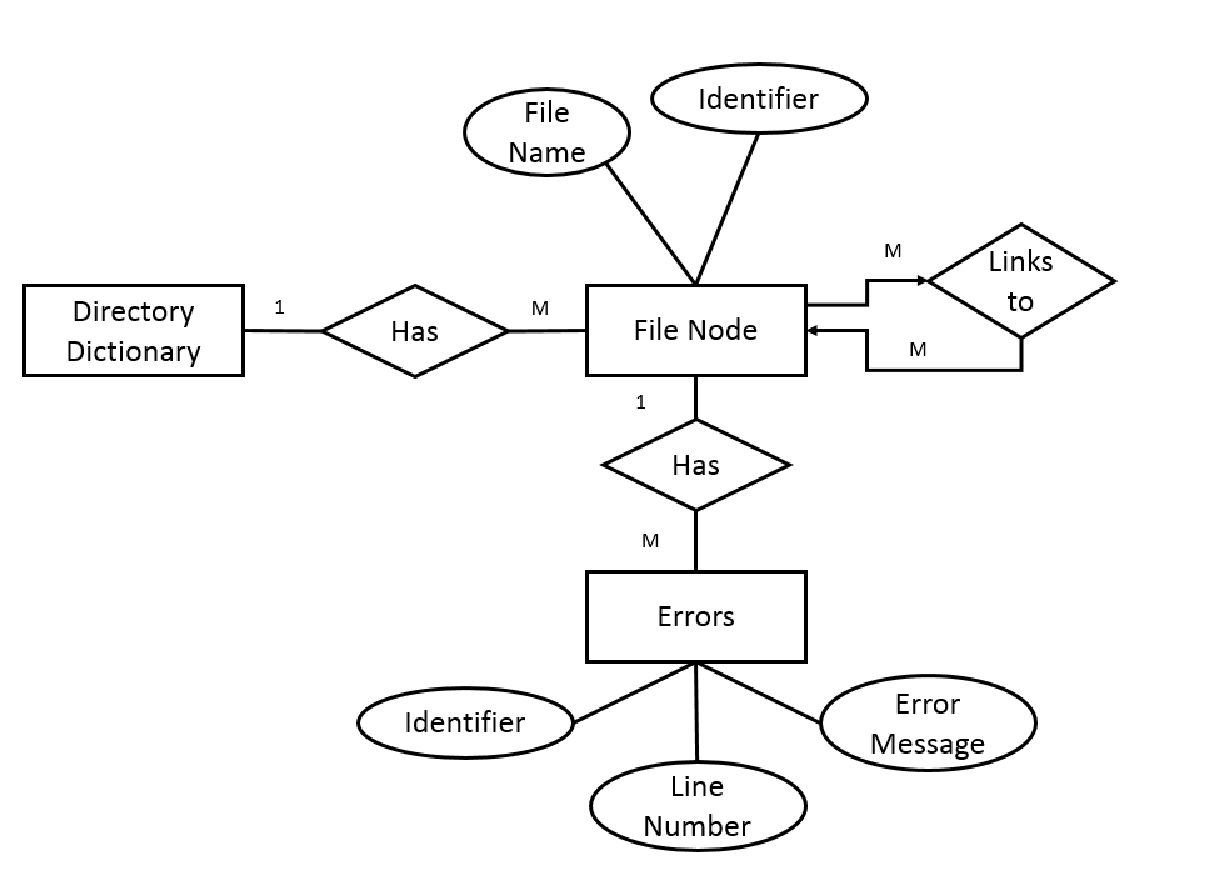
\includegraphics[width=.75\textwidth]{InformationERDEPS-eps-converted-to}
	\caption{Control flow of the way the data structure is formed}
\end{figure}

On execution of a Visual Studio Code command, the Electron application will activate the parser generate the file map. 
The visualization is done in the separate Electron window that is opened.
It has several things to display from the parser information. 
The main piece of information that the visualization displays is the file map and other information is the notification list. 
The file map is a graphic representation of the of the user's project solution. 
It appears as a hierarchical graph of interconnected nodes where the nodes represent a file or directory in the user's project directory, and an edge represents some link (defined in the parser section) between the two files. 
The location of the nodes in the hierarchy will reflect its position in the project's directory. 
This web will feature nodes of different sizes and will allow the user to zoom and pan the view. 
The size of the node is based on the number of links to that object.
A color corresponding to the type of file. 
Color values are based on the VSC color scheme for aesthetic reasons.
The name of the node is retrieved from the file struct name field and is displayed as text beside the node. 
A red circle will appear on the node if there are notifications within the FileStruct for that node. 
In other words, if the size of the notification array within the FileStruct is not zero. 
The file map is rendered within its own div using the vis.js library 'Network' module. 
The Library by default includes the rendering, panning and zooming functionality. \\

The other piece of the projects custom UI is the notification list. 
The notification list will display all notifications currently in the project directory in the form of a vertical list. 
These notifications will be retrieved when the UI opens from the same data structure is being generated. 
These notifications will be retrieved in a per node fashion and will also be grouped in the error list in the same order.
The notifications list will exist to the side of the file map in the same electron application screen. 
The list will allow the user to scroll when the number of errors result in the list exceeding the electron window height.
When a notification in the list is hovered over, these errors highlight the corresponding node in the file map by changing the color value of said node.
When a notification in the list is clicked, the extension will open the file in Visual Studio Code?s text editor and scroll to line where the notification location exists. 
The notification list is in its own div and has included scrolling functionality. \\

\begin{figure}[H]
	\centering
	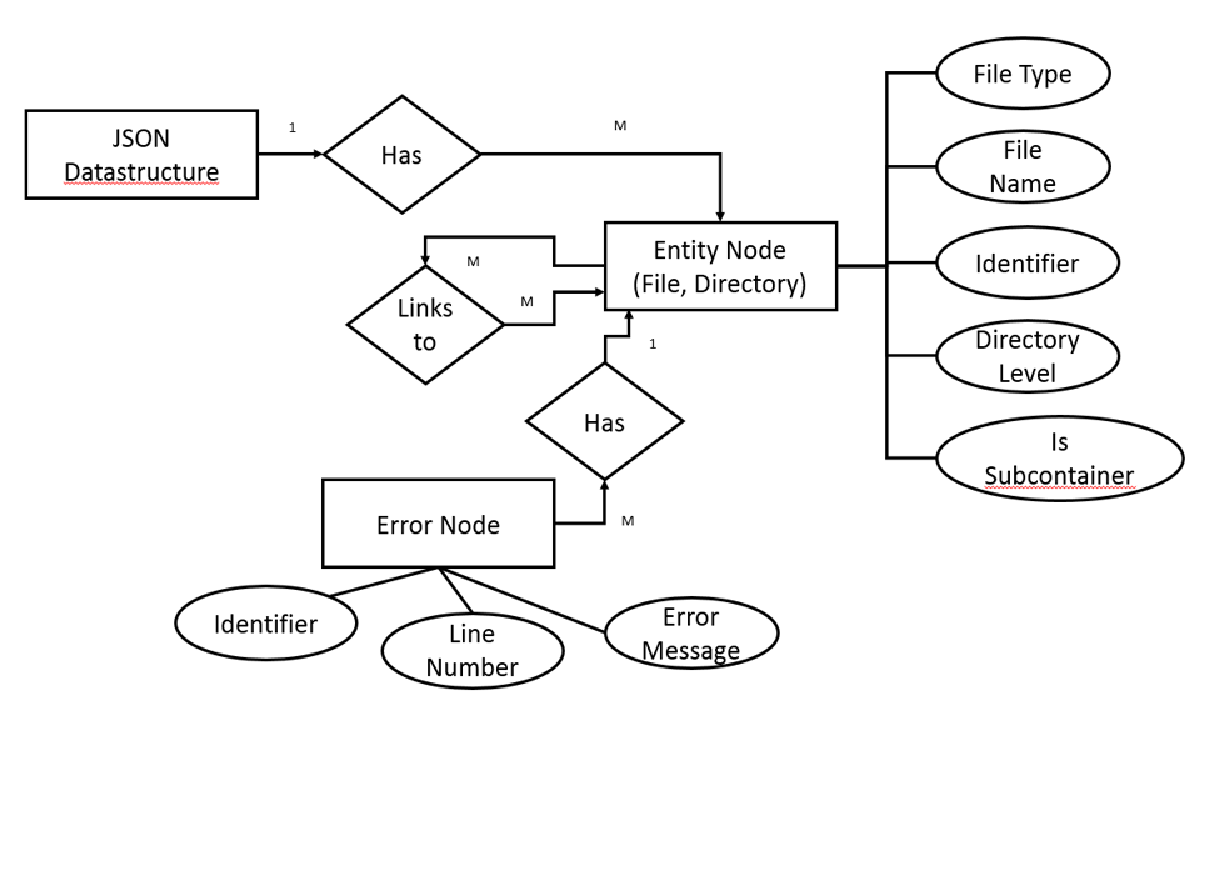
\includegraphics[width=.75\textwidth]{UpdatedDataStruct-eps-converted-to}
	\caption{Information that is stored in the data structure and the way that is it interpreted by the custom UI and displayed}
\end{figure}

Data handling within the Postal Extension consists of three main entities or processes: the data structure, serialization of the data structure and the storage of the data structure in a JSON file.
The data structure is a dictionary of file nodes, stored as JavaScript objects. 
These JavaScript objects come from the Parser parsing the currently loaded project for links and notifications.
The data structure can be considered the live version of the project data, as its data structure is updated by the parser every time the project is parsed. 
The nodes changed in the data structure will then be serialized into JSON jQuery using the JSON.stringify function built into JavaScript. 
This JSON will be saved to a file, which can further be read by the Electron UI functions for updating the project node and notifications visualization. \\

Now onto the IDE. 
There are two main interactions that happens the specific IDE events the opening of the custom extension UI and the interfacing network that allows the user to click on the custom UI in electron and have events happen in the VSC interface. 
The first of these events is opening the custom extension UI, this is done by creating a new process that runs the Electron window and passing the information that the parser has collected to that process.  
The interfacing network is opened and closed every time the user clicks a UI element within the custom UI. 
The network is a simple server client network with the server being the VSC IDE and the client being the Electron window. 
The VSC initializes itself as a server that will listen for the Electrons message when the user interacts with a UI Element. 
Once that happens the extension will navigate the users code window on VSC to the appropriate location that the user specified when they clicked on the custom UI.  \\

% What is its structure?
\subsection{Structure}

The extension is developed with a Model View Controller design.
The Model being a data structure that is created by the parser. 
The View being the custom UI displays a visualization of the data structure.
The controller is the communication between the data structure and the UI.

\begin{figure}[H]
	\centering
	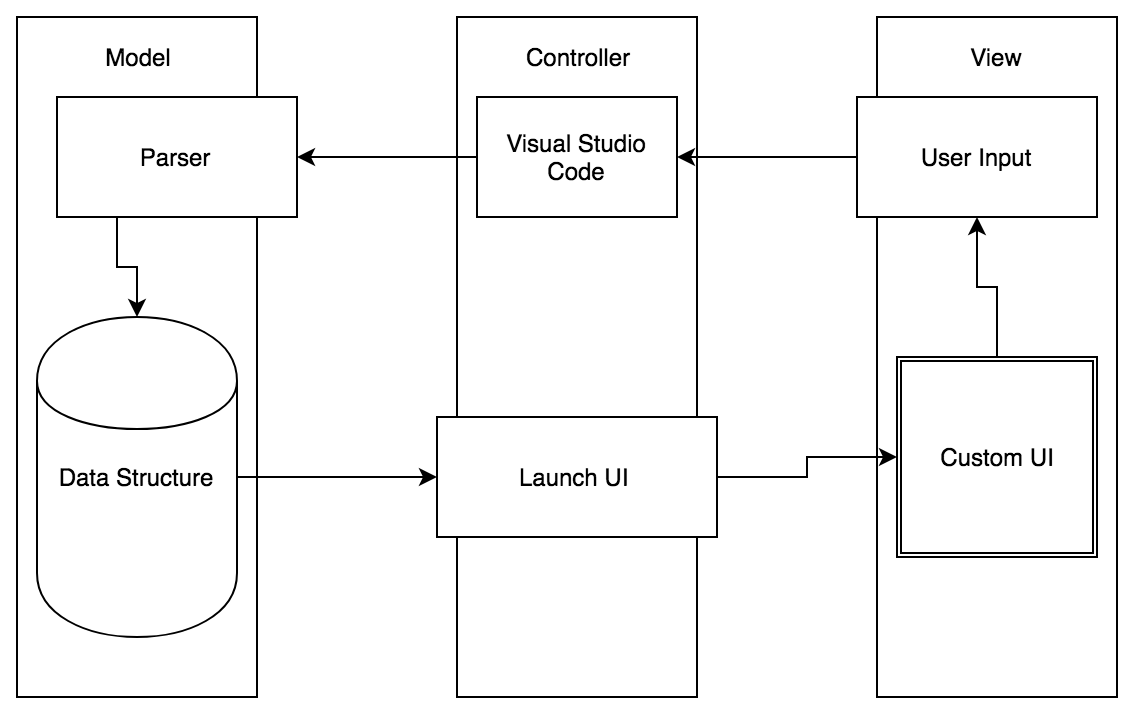
\includegraphics[width=.75\textwidth]{MVCsimple}
	\caption{Diagram of the way the Model View Controller Design is implemented}
\end{figure}

% Theory of operation: is a description of how a device or system should work
\subsection{Theory of Operation}

Once installed and with the proper grammars made for the project that the user is working on the extension should function as follows. 
The user can then use the command \texttt{command + shift + p} to open the command dialogue.
From there the user can input the \texttt{Postal} command. 
This operation will start the parsing of their files, and the creation of the custom UI that will open soon after inputting the command. 
Within the custom UI the user can navigate around the representation of their code using their mouse and zoom functionality.
They will be able to view different code elements based on the grammars they have defined.
The user is also able to view the notification list. 
The user can click on any of the nodes or any of the notifications and they will be navigated back to the VSC window where a new tab will be opened and the area in the code that was specified by the element clicked will be displayed, and ready for the user to edit.
The user is able to access and edit their custom grammars in the settings.json file that is part of VSC. 


% How does one install your software, if any?
\subsection{Installation}

\subsubsection{From Visual Studio Code Marketplace}
\begin{enumerate}
	\item	Within Visual Studio Code, click the extensions tab (the last one that looks like a block)
	\item 	type "postal" into the search bar
	\item 	click the install button
	\item 	Navigate to: \texttt{~/.vscode/extensions/postal-team.postal-\$version/}
	\item 	Run the command \texttt{npm install}
	\item 	Navigate to: \texttt{~/.vscode/extensions/postal-team.postal-\$version/lib/app}
	\item 	Run the command \texttt{npm install}
\end{enumerate} 

\subsubsection{From GitHub} Run the following commands:
\begin{enumerate}
	\item 	\texttt{git clone https://github.com/slichlyter12/Postal.git}
	\item 	\texttt{cd postal}
	\item 	\texttt{npm install}
	\item 	\texttt{cd lib/app}
	\item 	\texttt{npm install}
	\item 	\texttt{cd ../..}
	\item 	\texttt{code .}
	\item 	VSCode should now be open with Postal's source code
	\item 	Hit F5
	\item 	Navigate to: \texttt{~/.vscode/extensions/postal-team.postal-\$version/}
	\item 	Run the command \texttt{npm install}
	\item 	Navigate to: \texttt{~/.vscode/extensions/postal-team.postal-\$version/lib/app}
	\item 	Run the command \texttt{npm install}
\end{enumerate}

% How does one run it?
\subsection{Run Instructions}

To run the extension once it is properly installed all on has to do is open VSC and open a project. 
From there the user uses the \texttt{Command + Shift + p} command and the VSC command dialogue will be open, and the user can then input the command \texttt{Postal} and the Postal Extension will start.

% Are there any special hardware, OS, or runtime requirements to run your software?
\subsection{Prerequisites}

To use the extension the user needs to have Visual Studio Code and be able to use the npm installer.
To be able to run the npm install means that they have to have Node.js installed. 
They need this for the commands that are described in the Installation section.
This is needed because the extension uses Electron to display the map that the extension builds, and Electron is too large to package and have put on the Visual Studio Code Extension Marketplace.


\section{Resources and Technologies}

The most complex technologies the team had to learn was Node.js and vis.js

\subsubsection{Node.js}
For learning Node we primarily used the Electron reference guide available here: 
\url{https://electron.atom.io/docs/}
This was the most helpful resource in figuring out how to build an extension for Electron as well as basic node process information. 
The section on the Electron API was especially helpful. \\

The team also made use of a couple github projects for reference purposes. 
The biggest help by a wide margin was the VSCode Color Picker made by Anseki.
\url{https://github.com/anseki/vscode-color/}
While the code was quite dense it was also essential in figuring out how to launch an Electron window from VSCode. 
It also gave the team some insight in how to better build the high-level structure of our extension. 
It is important to note that the team did not take any code from the project and only referred to it as a guide for using the correct Node and Electron functionality. \\

\subsubsection{Vis.js}
Vis.js is intuitive for doing basic things with graph visualizations. 
However, it can be very clunky when trying to implement more complex behaviors on top of its standard functionality. 
The main resources used for figuring out Vis.js related difficulties were the official documentation and examples webpages.
\url{http://visjs.org/docs/network/}
\url{http://visjs.org/network_examples.html}
The documentation itself was helpful for more specific information like finding function overloads but was not at all useful for understanding how to use Vis.js's functionality. 
Fortunately, Vis.js also provided a very comprehensive examples page with samples demonstrating the majority of supported functionality and function usage. \\

\subsubsection{Additional Resources}
We also made use of other technology specific websites and Stack Overflow for minor issues.
Both Regex101 and Curious Concept's JSON formatter were very helpful tools.
\url{https://regex101.com/}
\url{https://jsonformatter.curiousconcept.com/}
Additionally, we based the majority of our parser’s architecture on the compiler we built in CS480. 
It was, in retrospect, surprising how useful that class was to completing this project.


\section{Learning and Overall Experience}
% What technical information did you learn?
% What non-technical information did you learn?
% What have you learned about project work?
% What have you learned about project management?
% What have you learned about working in teams?
% If you could do it all over, what would you do differently?

\subsection{Sam Lichlyter}
\subsubsection{Technical Information}
Since my main source of income over the past seven years or so is as a web developer, I am extremely familiar with JavaScript.
However, I had never used TypeScript before, which is essentially Microsoft's version of JavaScript that has a few added functionalities, including types.
I found this extremely helpful as one of my main complaints with JavaScript is that it is not typed.
I also learned how to use Node.js which I had been meaning to do for quite some time.
I had never heard of Electron before which was pretty useful to be able to essentially write a website that would be run as it's own application in it's own window.
This project also turned out to be a compilers crash course.
The parser we wrote was essentially a customizable compiler, so I learned a lot of the intricacies of how those work.\\

\subsubsection{Non-Technical Information}
I think one of the biggest things I learned was how much I appreciated some of the things we were taught in the very beginning of our college career that I more or less disregarded when they were first introduced to me.
The big one that stands out is paired-programming.
I don't think this project would have been as successful as it was or completed in the time frame needed without paired-programming.
Eric and I were able to successfully do this by him ``directing'' and me ``driving.''
I was able to focus on the syntax and typing while Eric was able to basically tell me how everything was connected.
If we had tried to do this on our own I don't think either of us would have been able to keep straight what had to be connected to what and we would have run into hours of debugging later down the road. \\

Another big thing I am now more appreciative of is designing before coding.
They tell us this all throughout our college career, but usually our assignments aren't big enough to warrant this kind of design first approach.
This project however definitely was.\\

\subsubsection{Project Work}
Piggy-backing a bit off of the last section, designing first is extremely important.
Especially for projects of this magnitude and bigger like I expect a lot of professional jobs will have us work on.
Our team didn't completely disregard designing the system before we started, we just didn't quite know what we needed, so it made it extremely difficult to design thoroughly. \\

\subsubsection{Project Management}
One of the biggest takeaways from this project about managing a team is communication.
It is extremely important that everyone is on the same page, and everyone knows what the end goal is.
This is something we ran into at least once.
At one point we were all on one page and our client was on another, and at another point some of us were on one page and the others were on a different page.
Keeping everything straight in a system like this is complicated, but everyone needs to know their roles and how they fit into the bigger picture of getting the whole team to where they want to be.\\

\subsubsection{Working in Teams}
This wasn't quite something I learned through this project but it was definitely exemplified in this project.
And that was that everyone on the team has their own strengths and weaknesses.
Some people are better at doing research into different technologies, others are better at conceptualizing large and complicated systems.
These are things that are vital to each team and that team should use these abilities and talents to their full extent. \\

Another important aspect I learned about working in teams was that separating business from pleasure is very important. 
At the end of the day you all want to be friends but still have a really cool project to show off to people.
You need to be able to separate personal feelings from what needs to get done, and then when the work is over, you need to not really talk about work until the appropriate time.
For me at least, I found this very helpful to maintain the friendships I had with the people on my team.\\

\subsubsection{What I Would Do Differently}
If I would do it all over again, I would go through the advice I just listed above and implement it.
I would put more effort into design first before implementation, make sure everyone knows their roles in the team and how they fit into the bigger picture, use the things we were taught in school for how they're meant to be used, etc. 

\subsection{Zach Schneider}
\subsubsection{Technical Information}
The core development of this project involved the learning and utilization of many new technologies, languages, and programming principles for the team and myself.
I had previously used VS Code, but had never developed an extension for it or any other Electron based code editing platform.
Debugging an add-on and testing it on all relevant platforms is not only useful practice for future projects in that vain, but also gives me a great appreciation for the work other developers have done over the years in extending the tools I use and enjoy.
This was my first foray into using TypeScript, a JavaScript super-set that includes types and class-based object oriented programming. I enjoyed working with TypeScript, and felt like it included many of the JavaScript programming strategies I'm familiar with while offering a more consistent and featured experience.
TypeScript was primarily utilized in programming for our Node.js server within VS Code.
I had used Node in one project previously, but our capstone project this year gave me a much more in depth view into how Node servers work and how to effectively program with them.
Additionally, I learned and became proficient in the Latex document preparation system.
Latex creates consistent, professional looking documents, and I used it to create most of the documentation and reports for this project. \\

\subsubsection{Non-Technical Information}
During this project I became more proficient in writing up formal documentation, particularly in adherence to IEEE standards. 
Learning how these kinds of documents are developed, updated and referenced will greatly aide me in all future programming jobs.
I also believe my writing ability improved overall, as the many different reports required for this class stretched me in ways I hadn't previously been challenged to attempt.
I learned how to merge the writing styles of others within a single paper in order to have a more cohesive submission that flows, instead of 4 separate sections pasted into one document.
Editing, while not re-writing is a skill of mine that has certainly been furthered while working on this project. \\

\subsubsection{Project Work}
Perhaps the most significant thing I learned about project design and implementation is how important it is for the designers and implementers to be on the same page.
Even in our case where each of our team members served both roles, we had quite a few problems early on in not understanding what design or project feature the others were trying to convey to us.
Sometimes we mistakenly wrote code in an entirely different train of thought than other sections, leading to serious conflicts in our project's structure and function.
Ultimately, our solution was increased communication and more time put into the planning stages of each component's section.
Along these lines, our team struggled to even conceptualize what we wanted from our project as a whole and if our concepts would actually work.
In a few cases, we wrote a design or specification for a feature, then realized while creating that feature that the original envisionment would not work out.
What I can take away from this is, again, how important the planning and design stages of projects are to their success.
Experience in working on projects like ours will help when starting on new projects in the future. \\

\subsubsection{Project Management}
One of the issues our project faced was running out of time at deadlines. 
Even if they were self-established deadlines, we couldn't strike a balance of having a deadline be significant while also flexible enough to accommodate series design problems that we occasionally encountered.
My time management in these contexts was certainly tested in trying to allow for enough time to accomplish what was needed while also not setting deadlines too far into the future.
Additionally, I learned the importance of differentiating when a feature or task should be done versus when it needs to be done. 
Setting these standards for myself and communicating them to my team effectively contributed positively to my knowledge of project management. \\

\subsubsection{Working in Teams}
Team work can often be difficult - personality clashes, differences in work ethic, lack of communication - these are all fairly expected when working on team projects. 
While our team was generally able to learn and work through many of these standard issues, a unique circumstance we possessed was that we are all friends outside of school.
Some of us had heard warnings to not work with friends on projects, but we didn't really pay them heed.
Throughout this project, it has been exceedingly difficult to draw the line between our work relationships and our social relationships. 
Often we would finish up work on the project then promptly spend the rest of the weekend hanging out.
While this led to an easy dynamic early on, our relationships became strained when serious problems occurred, such as individuals not meeting deadlines, not communicating or forgetting about meetings.
Though our project worked out in the end, this experience is not one that I'd like to undertake with friends again.
In the future I will aim to let friends be friends and work colleagues be work colleagues. \\

\subsubsection{What I Would Do Differently}
With the aforementioned lessons being learned, if I were to do this project again, I would do a few things differently.
First, I would not choose to work with close friends on an extended and stressful project such as this.
I would make sure to spend a more significant amount of time in the early stages really nailing down what the project's purpose, goals, design and features will be.
Communication about these plans would be made with the team and our client much more frequently at the beginning.
Coding would begin in early December instead of January, as the extra month of working through bugs would make a large difference in final quality and lessen deadline stress along the way.
Finally, I would begin utilizing user testing far earlier, even before features are complete in order to get feedback and save the team some of the re-writing that occurred in the later phases of the project.
Despite these changes I would make, I feel the majority of the project went well and I'm proud of the result.

\subsection{Cramer Smith}

\subsubsection{Technical Information}

This was the largest project that I have ever made, and we wrote it in JavaScript and TypeScript. 
I learned a lot about JavaScript and Node.js.
I learned the usefulness of code organization. 
I always knew that having well organized code was good, but I had never had a long term large project that really needed it.
It was great after we had done a major part of the development adding smaller features to the tool was much easier because we already had all these small pieces well put together and these parts could easily be put together to make something larger.
I also learned about thenables. 
Thenables are a very annoying and incredibly flexible way of working with asynchronous function calls.
I had never used TypeScipt and for any function that was not working as I expected is because it was probably running asynchronously. 
To fix it I quickly learned that a thenable was needed.
I also learned about using a client server relationship to communicate between processes.
To get the user events between the custom UI with the Electron window and the VSC editor we needed to communicate between two different processes. 
I always though that processes were very closed off entities, and they are unless you tell the processes to communicate to one another. 
To do that communication I set up the client server. \\

\subsubsection{Non-Technical Information}

I learned some self confidence.
Usually in team project I do not try to be the idea man. 
I have always assumed that others are smarter than me, but this project I learned that I have some good ideas.
So I tried to make myself more heard during this project. \\

\subsubsection{Project Work}

It is a lot of work to get a big project working, and a lot of work can be saved by a good initial design.
We had an okay initial design. 
The core ideas of that initial design are still there, but some of that design did not work as expected. 
We had to redo a lot of work because of the initial design was not sufficient.
But even if we had had a perfect design it would still have been a lot of work. 
The amount of hours that we put in to get the tool working, was more than I thought it would be. \\

\subsubsection{Project Management}

Communication is extremely important. 
I knew that before.
It was really evident though when we initially delegated the separation of work between the four of us, and we all started developing without talking too much to one another. 
Then by the time we were all supposed to be done with our respected parts we came together and none of the parts worked together. 
We should have been talking with each other more in that crucial development phase.
That being said
I think I would have liked some more structure with the way we all managed the project. 
It was nice when we nominated the team leader to handle all the document deadlines.
It was nice to know that if I was unsure of what I needed to do for X document I could ask Zach.
That was the only real structure that we had though. \\	

\subsubsection{Working in Teams}

It is hard to not have emotions rise.
There were times when it was very tense in out Slack chat. 
I am still not sure how to remedy this problem.
I think it would be different in a professional environment.
I delegation is good, but only with really good communication.
There needs to be a good understanding of the expectations of the team. \\
 
\subsubsection{What I Would Do Differently}

Besides the differences that I stated in the above sections I wouldn't be in a team with my friends. 
I think this hurt my friendships with these people, and I was probably less motivated because I knew my friends would be more forgiving. 


\subsection{Eric Winkler}

\subsubsection{Technical Information}
From a technical perspective, I've learned about or become more proficient in:
\begin{itemize}
    \item JavaScript and TypeScript
    \item Node.js
    \item Electron
    \item Vis.js
    \item Git and Github
    \item Other Web-technologies (HTML, CSS)
    \item Software Design
    \item Asynchronous design
    \item Object oriented Programming
    \item Debugging
    \item Compilers
    \item Using APIs in general
    \item Reading Documentation \\
\end{itemize} 

\subsubsection{Non-Technical Information}
The theme to the non-technical lessons I've learned while working on this project is that I have a new appreciation for a ton of things I learned here but hadn't used in a practical way before. \\

To start with, I now love paired programming. 
Building the Parser and back-end of this project was potentially the most complicated thing I have attempted during my undergraduate career. 
It was almost necessary to have Sam writing code while I focused on keeping track of what exactly we were doing and what we still had to do. 
Writing most of the code together probably saved us tens of hours. \\

I also learned to love classes. 
I've never had to use classes on the basis of trying to abstract complex problems but being able to describe things in terms classes and forget about lower level details was very helpful. \\

Finally, I learned to appreciate the importance of designing before coding. 
I'm not sure I've ever completed a homework assignment by first designing it before writing the code. 
Everything had been, relatively speaking, simple to implement. 
However, without an assignment guide or anyone to hold our hand through the process, we were forced to actually draw out the components of the system and really think about why we were implementing things the way we were.
I think the most valuable piece of non-technical Information I gained from this project would be that I really like to do design related work. 
I may attempt to pursue a career path where I can do more architecture and systems design than programming, provided that exists. \\ 

\subsubsection{Project Work}
The most valuable lesson about project work I learned is that if a group plans on splitting the work into separate modules and assigning one or more modules exclusively per person, said modules should still be designed together as a group. 
The team has mentioned this problem before in previous documents and it should be mentioned again how important it is to have well defined interfaces. 
What I've never brought up is that those interfaces imply that the design and functionality of the two modules are already clearly defined and understood by the team.
That's the more important lesson to note. 
It doesn't matter at all what the exact specifications of the interfaces are if there is missing or overlapping functionality in those modules. 
If I had to come away with only one important lesson from this project it would be this: design thoroughly with all members of the team present.\\

\subsubsection{Project Management}
From a project management perspective, I've learned the importance of setting one's own deadlines and setting them early. 
Around the middle of winter term, the team concluded that we were starting to fall behind of where we wanted to be in terms of implementation progress. 
We had made the decision to get a working build of our extension on the VSCode store by the next coming Monday. 
Nothing was specifically due for the class but we had placed this artificial deadline on ourselves because of concern that something might cause problems if we had planned to be finished by the end of the term instead. 
Because of the how tight our deadline was, we forced ourselves to work close to 36 hours within a three-day period. 
During that crunch we discovered serious problems with our design that would have caused the project to be a failure if we had waited much longer.
My opinion is that deadline may have saved the project.\\

\subsubsection{Working in Teams}
I was fortunate to work with an excellent team. 
Everyone was motivated and completed their assignments on time. 
We had no major problems and communication was consistent. 
One lesson I learned is that it helps quite a bit to have at least one person who can act as a leader. 
This person doesn't necessarily have to delegate jobs or roles, but having an individual to check on team member's progress and keep a general level of organization is beneficial. \\

 
\subsubsection{What I Would Do Differently}
A problem the team had that we don't reflect on much is that we had a bit of miscommunication on project priorities with our client. 
We had spent so much time on our back end figuring out how to get our parser working consistently that we had neglected the front end quite a bit. 
In a meeting our client was not happy with our progress, though a substantial amount had been made since our last check in. 
We had failed to realize that as a tool, it was only as good as it was usable, i.e. its front end. 
I regret not frequently communicating with our client and making him a larger part of the process.\\


\pagebreak
\section{Appendix 1}
\subsection{Code Samples}
	\subsubsection{Example Grammar}
	This is the default grammar that parses HTML and PHP files for divs and links.
	
	\begin{lstlisting}
"Postal.grammars": [
        {
            "title": "div",
            "type": "tagged",
            "filetypes": [
                "html",
                "php"
            ],
            "options": {
                "tagStart": "<div",
                "namedOption": "id=\"(.+?)\"",
                "tagEnd": ">",
                "closingTag": "</div>",
                "nodeColor": "blue"
            }
        },
        {
            "title": "href link",
            "type": "link",
            "filetypes": [
                "html",
                "php"
            ],
            "options": {
                "link": "href=[\"](.+?)[\"]",
                "nodeColor": "blue"
            }
        }, ...
]
	\end{lstlisting}

	\pagebreak
	\subsubsection{Recursive Get All Links}
	This function grabs all the links from the data structure of a specified file struct and it's children.
	\begin{lstlisting}
// Recursive function to get all links from this and children
function getAllLinksFromFileStructRecursive(FileStructID) {
    var links = [];

    // check parent
    if (DFS[FileStructID].links.length > 0) {
        for (var i = 0; i < DFS[FileStructID].links.length; i++) {
            var link = DFS[FileStructID].links[i];
            links.push(link);
        }
    }

    // check children
    if (DFS[FileStructID].subContainers.length > 0) {
        var childLinks = [];
        for (var i = 0; i < DFS[FileStructID].subContainers.length; i++) {
            var childFileStructID = DFS[DFS[FileStructID].subContainers[i].toFileStructid].id;
            childLinks = getAllLinksFromFileStructRecursive(childFileStructID);

            // push what we found to parents link list
            for (var j = 0; j < childLinks.length; j++) {
                links.push(childLinks[j]);
            }

        }
    } 

    return links;
}
	\end{lstlisting}

\pagebreak
\section{Appendix 2}	
\subsection{Images}
	\begin{figure}[H]
		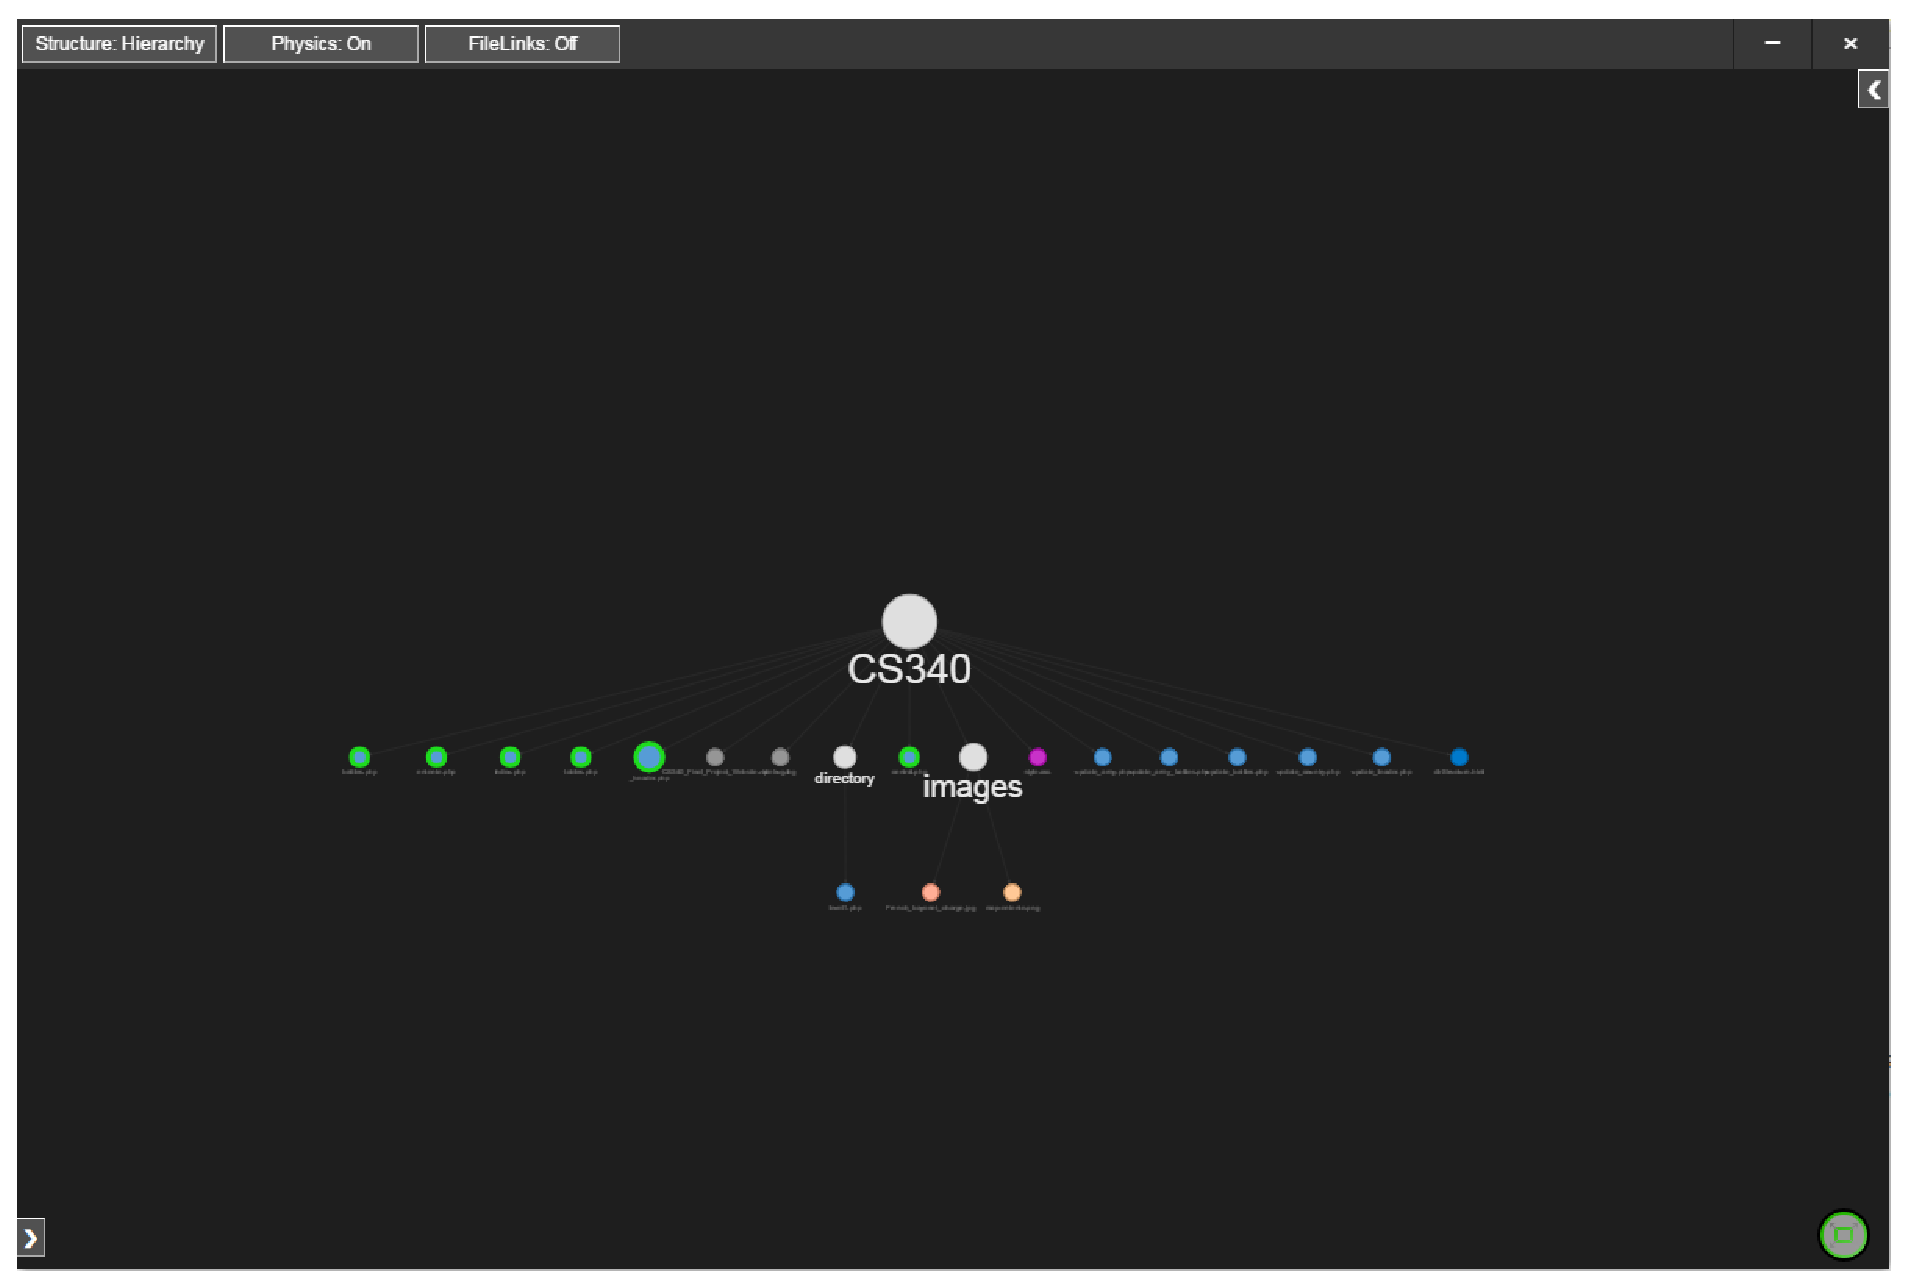
\includegraphics[width=500px]{PostalUI}
		\caption{Visualization Interface}  
	\end{figure}
	
	\begin{figure}[H]
		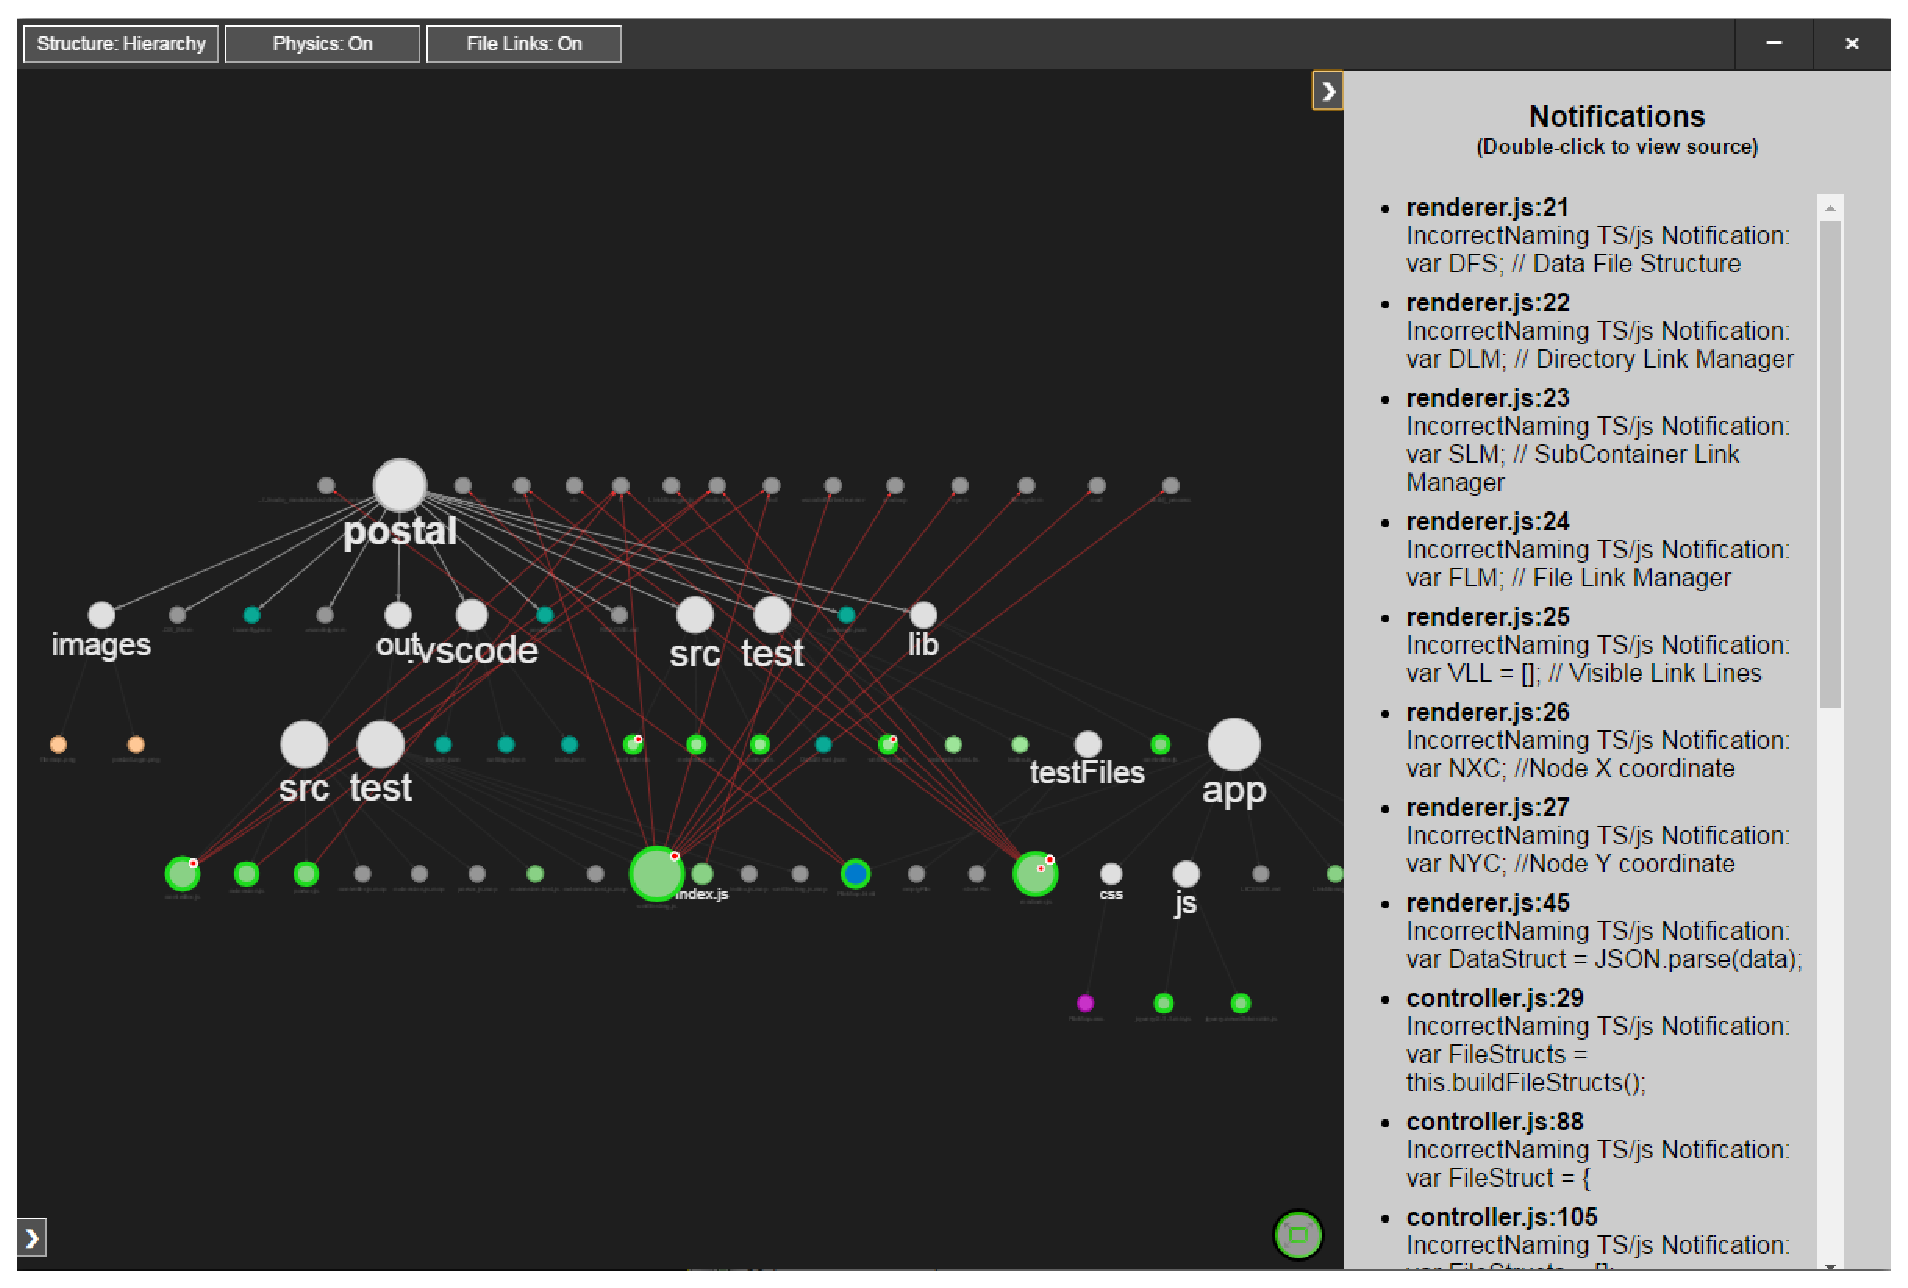
\includegraphics[width=500px]{PostalNotification}
		\caption{Notification Interface}  
	\end{figure}
	
\pagebreak
\bibliographystyle{IEEEtran}
\bibliography{progress-report-team38}


\end{document}

